\section{Output simplu}
\label{sec:output simplu}
La sfârșitul capitolului anterior, ai făcut cunoștință
cu primul tău cod PHP:
\lstinputlisting{cap01/info.php}

Prima linie marchează începutul procesării PHP. Ce se află
înaintea \texttt{<?php} este trimis așa cum este către client.
Hai să testăm. Scrie ceva în tagul <h1> înainte de începutul
procesării PHP și vezi ce iese:
\lstinputlisting{cap02/1-helloinfo.php}

PHP generează prea mult cod HTML pentru gusturile noastre simpliste, deci
fă cunoștință cu un cuvânt cheie în PHP: \texttt{echo}. Sintaxa
generală este:
\begin{verbatim}
echo <EXPR>;
\end{verbatim}
unde \texttt{EXPR}  trebuie să fie o expresie care evaluată, se reduce la o valoare.

\attention{Nu te speria dacă nu înțelegi totul, voi reveni asupra subiectului. Deocamdată urmează pur și simplu pașii prezentați de mine, respectând sintaxa.
Simte-te liber să faci modificări, să experimentezi. Dacă faci ceva ce generează
o avertizare sau o eroare nu te impacienta, citește-o cu atenție, încearcă
să o înțelegi, și cere lămuriri pe wiki-ul proiectului.
}

Hai să-l învățăm pe PHP să ne salute. În notepad++ crează un nou fișier
și salvează-l ca \texttt{salut.php} în htdocs, apoi introdu codul:
\begin{lstlisting}
<?php
echo 'Salut Flavius';
\end{lstlisting}
Acum fă cu telnet o cerere HTTP, să vezi exact ce se întâmplă atunci când
interpreterul PHP execută acel cod:
\begin{verbatim}
GET /salut.php HTTP/1.1
Host: localhost
\end{verbatim}

Ce observăm? Exact! Observăm că nu vedem nici urmă de cod PHP, vedem doar
outputul generat de el. Nu tu \texttt{<?php}, nu tu \texttt{echo}. Asta
ne demonstrează că PHP ne-a procesat scriptul, script care a generat
output. Dacă scriptul nu ar fi generat output, \textit{response body}-ul
HTTP ar fi fost gol.

În al doilea rând, \textsl{http response body} nu conține date în format HTML.
De ce? Simplu, deoarece nu i-ai spus niciunde să genereze nimic ce ar putea arăta a
HTML. Cum facem asta? O posibilitate ar fi următoarea:
\begin{lstlisting}
<?php
echo '<html><body>';
echo 'Salut Flavius';
echo '</body></html>';
\end{lstlisting}

Concluzia pe care o tragem este că PHP habar n-are ce este HTML. De ce?
După cum am spus atunci când ai instalat CLI-ul PHP (numit \texttt{php.exe}),
PHP este un limbaj de scripting general. De fapt nu este legat în niciun mod de
HTML sau de site-uri. Este doar felul în care îl folosim noi și majoritatea
restului lumii. De fapt, PHP poate genera orice, imagini, documente, animații
(flash). Chiar nu ești restrâns la HTML, dar nici nu te ajută în acest sens --
trebuie să scrii manual codul HTML, după cum ai văzut mai sus.

Vei vedea însă că îți pune la dispoziție constructe care înlesnesc generarea
de HTML -- de exemplu poți genera o galerie de imagini aflate într-un anumit
director pe server, fără să trebuiască să știi dinainte numele fișierelor.

Totuși exemplul nostru anterior nu prea are sens -- nu este nimic dinamic în el.
L-am putea rescrie la fel de bine doar în HTML static, însă deoarece
vreau să demonstrez altceva, voi genera totuși mesajul de salut cu PHP:
\begin{lstlisting}
<html>
	<body>
		<?php
		echo 'Salut Flavius';
		?>
	</body>
</html>
\end{lstlisting}

Observi că pentru a termina procesarea PHP și a afișa din nou totul
așa cum este (en. \textsl{unparsed}) se folosește \texttt{?>}.
În acest mod poți porni și opri procesarea PHP de oricâte ori dorești în același fișier.
La sfârșitul fișierului procesarea este terminată automat, de aceea în exemplele
anterioare nu a fost nevoie de {\glqq}?>{\grqq}.

\attention{Mai observă și cum mi-am făcut codul ușor de citit \textsl{indent}ându-l (en.
\textsl{to indent}), adică am aliniat deschiderea fiecărui tag HTML cu tag-ul
de închidere corespunzător, făcându-mi codul lizibil. Pentru codul nostru sursă
minuscul nu prea contează, însă diferența de mentenabilitate va fi
vizibilă când fișierele vor avea sute sau mii de linii de cod (LOCs en.
\textsl{lines of code}). Deci obișnuiește-te
să indentezi codul apăsând tasta \keystroke{TAB} pentru fiecare nou nivel de
indentare necesar.}

Din acest punct înainte scopul nostru este să învățăm PHP, nu să generăm
cod HTML valid, deci nu ne vom mai obosi să decorăm textul generat
cu \texttt{html} sau \texttt{body}. Însă nu uita că într-o pagină HTML
normală, validă, și asta trebuie făcut, eventual
punând și un
\textsl{doctype}\footnote{
\href{http://en.wikipedia.org/wiki/Document_Type_Declaration}{document type declaration}}, altfel
browserul intră în \href{http://en.wikipedia.org/wiki/Quirks_mode}{quirks mode}.

%----------------------------------------------------------
\section{Folosirea variabilelor}
Înainte de a trece la noțiuni noi, trebuie să revenim asupra exemplului nostru
cu câteva completări:
\begin{lstlisting}
<?php
echo 'Salut Flavius';
\end{lstlisting}
Știm deja că \texttt{echo} este un cuvânt cheie care generează output pe baza
primului său parametru. Sper că ai intuit deja că fiecare instrucțiune
trebuie separată de următoarea prin ';'.

Însă ce este 'Salut Flavius'? Este o valoare în primul rând, pentru că
i-o putem pasa lui \texttt{echo}. În al doilea rând, este o constantă,
deoarece nu se modifică. La fiecare interpretare a scriptului, \textit{output}-ul
va fi același. Sumarizat: este o \textsl{valoare constantă}.

Pe lângă faptul că este o valoare constantă, mai este și un \engl{șir de caractere}{string}.
Acesta este motivul pentru care
am pus mesajul între apostrofuri -- altfel PHP ar fi încercat să
interpreteze \textsl{Salut} și \textsl{Flavius} ca constructe ale limbajului,
care evident nu există.

\good{Corect terminologic spunem deci că 'Salut Flavius' este un \textit{string constant} sau
mai pe larg \textit{o valoare constantă de tip string}.}

Deci încearcă! Fă-l pe PHP să genereze erori:
\begin{lstlisting}
<?php
echo Salut Flavius;
\end{lstlisting}
Mesajul de eroare ne-ar putea părea confuz:\\
\texttt{Parse error: syntax error, unexpected T\_STRING, expecting ',' or ';'}\\
Ceea ce se întâmplă este următorul lucru: PHP citește \texttt{echo}, și deoarece a citit
și a recunoscut instrucțiunea \texttt{echo}, intră în contextul semantic în care se așteaptă ca următorul
lucru să fie o valoare, însă nu găsește una, ci întâlnește \texttt{Salut},
pe care nu-l recunoaște\footnote{De fapt, parserul se blochează la {\glqq}Flavius{\grqq}, însă
ca să explic asta cum trebuie, ar fi trebuit să fi introdus deja constantele}
ca și construct al limbajului.
De aceea ne spune că nu se așteaptă să vadă T\_STRING-ul \texttt{Salut}.

Dar stai puțin, de ce îl numește {\glqq}T\_\textbf{STRING}{\grqq}, dar nu îl acceptă ca string?
Pentru a înțelege asta, trebuie să privești puțin lucrurile din perspectiva parserului
PHP. Codul sursă pe care îl scriem în limbajul PHP este folosit ca input pentru
parser. Acest input scris de noi este citit de PHP ca string, ca un șir de caractere.
Din acest motiv PHP ne spune foarte corect că nu se așteaptă să vadă acel string acolo,
ci altceva.
\attention{Pentru PHP, codul scris de noi este un simplu text.}
Hai să vedem ce ar genera PHP dacă nu s-ar aștepta să vadă un string
din perspectiva noastră:
\begin{lstlisting}
<?php
echo 'Salut' 'Flavius';
\end{lstlisting}
ne zice \texttt{Parse error: syntax error, unexpected T\_CONSTANT\_ENCAPSED\_STRING}.

Ce înveți din asta? În primul rând, înveți că mesajele de eroare, deși nedorite,
oferă informații prețioase despre ce s-a întâmplat. Din proprie experiență
pot spune că vederea unui mesaj de eroare sau avertizare e ca o mână cerească,
reversul medaliei fiind mult mai frustrant: să nu vezi o eroare, dar codul
nici să nu funcționeze așa cum îți imaginezi că ar trebui să funcționeze -- sau
mai rău, să nu afișeze nimic, lăsându-te în întuneric complet. Deci fi fericit
când PHP îți spune ce ai greșit, caută să înțelegi ce-ți spune, și apoi
repară-ți greșeala.

Pe lângă stringuri, mai există și alte tipuri de valori constante. PHP înțelege
\engl{numere întregi}{integers}, de exemplu \texttt{42},\footnote{Sunt curios
când va veni cineva să-mi spună de ce am ales 42 :-)}
numere cu virgulă (en, \textsl{floating point numbers} sau scurt \textsl{floats}),
unde partea zecimală
e separată de partea întreagă prin punct, de ex \texttt{3.1415}, și alte lucruri
asupra cărora vom reveni. Hai să ne uităm la un exemplu:
\begin{lstlisting}
<?php
echo 'Salut 00';
echo 7;
echo '. PI este ~';
echo 3.1415;
\end{lstlisting}

\subsection{Variabile și tipuri de date elementare}
Toate bune și frumoase cu lucrurile cu care ai făcut cunoștință
până acum, însă ele nu te-au ajutat să creezi ceva dinamic.

Deci hai să facem un pas înapoi și să ne gândim ce înseamnă și
ce implică o eventuală dinamicitate. Pentru a fi dinamică, o
pagină trebuie să fie capabilă să primească date de intrare (\texttt{input}),
pentru a genera date de ieșire (\texttt{output}) pe baza acestora.

De exemplu, să zicem că vrem să facem o pagină care în loc să afișeze
mereu {\glqq}Salut Flavius{\grqq}, afișează {\glqq}Salut <nume>{\grqq}. Acest input (numele) trebuie
salvat undeva, altfel nu avem acces la el. Bine ai venit în lumea variabilelor.

O variabilă are trei caracteristici
\begin{enumerate}
\item un \textsl{nume} sau \textsl{identificator}
\item o \textsl{valoare} pe care o ține
\item \textsl{tipul de date} (en. \textsl{datatype}) al valorii\footnote{mai
spunem colocvial și \textit{tipul de date al variabilei} însă în PHP tipul
de date este inerent valorii -- vom reveni mai târziu asupra acestui aspect} precum
string, int sau float pe care le-ai cunoscut mai devreme
\end{enumerate}

Identificatorul variabilelor începe mereu cu \$, primul caracter după el
trebuie să fie o literă sau underscore (\_), iar următoarele
caractere pot fi litere, cifre, sau underscore.
Nu există o limită în lungimea identificatorului, și nici restricții privind
numirea lor. Există însă reguli nescrise pe care le vei întâlni mai târziu,
cât și variabile pe care PHP le crează automat pentru tine.

Valoarea unei variabile poate fi orice bucată de informație ce poate
fi salvată.

Tipul de date al valorii poate fi unul din cele trei prezentate mai sus,
sau altele pe care le vom cunoaște în acest capitol și în capitolele următoare.

După cum am spus, \texttt{echo} afișează valoarea unei expresii.
Această valoare poate fi una constantă, precum în exemplele anterioare,
însă poate fi și o variabilă. Exemplu:
\lstinputlisting{cap02/3-hello-var-error.php}
PHP ne va atenționa cu o notificare că am încercat să accesăm o variabilă
nedefinită. Pentru a defini o variabilă trebuie să-i atribuim o valoare
mai întâi, iar asta o facem cu \textsl{operatorul} de atribuire \textsl{=}.
Putem spune și că \textit{am salvat valoarea X în variabila Y}. Exemplu:
\lstinputlisting{cap02/4-hello-var.php}

\attention{\texttt{echo} nu adaugă automat spații niciunde. Este responsabilitatea
noastră să o facem. PHP chiar nu are noțiunea de {\glqq}cuvinte{\grqq}. Pentru el, un
șir de caractere este un șir de caractere și atât.} 

În cazul de față, variabila \texttt{\$nume} nu prea își are rostul, deoarece o
folosim o singură dată. Însă imaginează-ți că ai un script lung,
și vrei să refolosești acel nume în diferite locuri în cadrul generării de
output. Variabilele sunt ideale pentru acest lucru, deoarece nu trebuie
decât să schimbi valoarea într-un loc, iar schimbarea va fi preluată în
întregul script:
\lstinputlisting{cap02/5-hello-var-reuse.php}

Felicitări, ai creat primul tău script care reutilizează variabile.

\subsection{Operații cu string, int, float}
Cu aceste tipuri de date se pot face operații. În primul rând,
stringurile pot fi \textsl{concatenate}, indiferent dacă sunt salvate
în variabile sau provin din valori constante. A concatena
înseamnă a lipi un string de următorul, pentru a forma un nou string.
Exemple:
\lstinputlisting{cap02/6-concatenare-stringuri.php}

\textit{Linia 2} face următorul lucru: mai întâi concatenează cele două valori constante
'Salut ' și 'Flavius', operație în urma căreia rezultă \textsl{valoarea intermediară}
'Salut Flavius'. Îți poți imagina că această valoare stă acum de partea
dreaptă a operatorului de atribuire. Iar deoarece avem o atribuire, această
valoare intermediară este salvată în variabila \texttt{\$a}.

\textit{Linia 3} afișează valoarea salvată în variabila \texttt{\$a}.

Ne-am fi putut folosi de acea {\glqq}valoare intermediară{\grqq} de pe linia 2 afișand-o direct:
\begin{lstlisting}
<?php
echo 'Salut ' . 'Flavius';
\end{lstlisting}
Aici valoarea intermediară \textit{care rezultă în urma concatenării} celor două stringuri
constante este pasată direct (ca o nouă valoare) instrucțiunii \texttt{echo}.

După cum ai observat pe \textit{linia 2}, operația de atribuire este interpretată
de PHP de la dreapta la stânga. Mai întâi sunt făcute rând pe rând operațiile
din partea dreaptă a atribuirii, apoi valoarea rezultată este salvată în
variabila aflată în stânga atribuirii. Datorită acestei ordini spunem că
operația de \engl{atribuire}{assignment} este \textsl{right-associative}.

\textit{Linia 5}: Datorită asociativității de dreapta a operației de atribuire,
într-o atribuire putem folosi o variabilă precum \texttt{\$a} în partea dreaptă, genera
o valoare temporară pe care o atribuim tot variabilei \texttt{\$a}, suprascriind
valoarea sa inițială. Dacă am fi știut că mai avem nevoie de nume ca valoare
de sine stătătoare, pe linia 5 ar fi trebuit să introducem o nouă variabilă
căreia să-i atribuim noua valoare,
astfel încât să nu pierdem valoarea inițială a lui \texttt{\$a}.
Însă în cazul nostru, \textit{linia 5} este extrem de curată,
deoarece nu introduce o nouă variabilă în mod inutil.

Să revenim la sintaxă și la semantică. Sintaxa lui echo este:\\
\texttt{echo <EXPR>;}\\
Iar a operației de concatenare este:\\
\texttt{<expr1> . <expr2>}\\
<expr1> și <expr2> pot fi orice fel de expresii, fie ele valori constante,
sau variabile -- deoarece variabilele au și ele o valoare pe care
o cară cu ele. În urma operației de concatenare rezultă o valoare
intermediară. Chiar dacă aceasta e {\glqq}invizibilă{\grqq} (deoarece
PHP o crează în mod transparent pentru noi), ea este tot o valoare ca oricare
alta, deci poate fi pusă oriunde PHP ne lasă să punem o expresie.

Dar stai puțin, operația de concatenare însăși acceptă două expresii!
Consecința? Putem concatena acele valori intermediare, transparente,
într-un lanț\footnote{În matematică spunem că abordăm problema
\href{http://en.wikipedia.org/wiki/Structural_induction}{inductiv}.}:\\
\texttt{<valoare1> . <valoare2> . <valoare3> . <valoareN>}

În astfel de cazuri, <valoare1> este concatenată cu <valoare2> și rezultă
o valoare intermediară, transparentă, care este apoi concatenată cu <valoare3>,
și tot așa.
Exemplu:
\lstinputlisting{cap02/7-concatenare-stringuri.php}

Despre limbajul PHP se spune că este \textsl{dynamically typed}. Asta înseamnă
că poate (în limitele {\glqq}bunului simț{\grqq}), să convertească automat
o valoare de un tip, într-o altă valoare de alt tip, care e cât
mai apropiată de valorea inițială. Așa se face că deși operatorul
de concatenare acceptă doar doi parametri de tip string, putem totuși
concatena și numere. PHP va crea însă încă o valoare intermediară
cu reprezentarea valorii inițiale ca string. Un exemplu:
\lstinputlisting{cap02/8-concatenare-inference.php}

\attention{Încearcă să eviți a-l forța pe PHP să
trebuiască să convertească un număr într-un string,
deoarece operația asta consumă resurse inutil.
În schimb folosește sintaxa alternativă a lui \texttt{echo}
cu care vei face cunoștință în continuare.}

\begin{Exercise}[title={Primul cod propriu}]
Continuă codul următor astfel încât să afișeze\\
\texttt{Valoarea lui PI este 3.1415.}
\lstinputlisting{cap02/9-ex-pi.php}
\end{Exercise}

Există o sintaxă alternativă pentru \texttt{echo}, care ne permite
să afișăm valori constante amestecate cu valori variabile fără
a mai crea valori intermediare, deci PHP poate executa
scriptul mai rapid și cu consum mai mic de memorie.
Pentru asta punem virgulă între valori:
\lstinputlisting{cap02/10-echo-list.php}

Asta înseamnă practic că \texttt{echo} va fi apelat asupra fiecărui
parametru din listă. Atenție: diferențele se pot vedea
doar atunci când lucrezi cu cantități mari de informație.

\begin{Exercise}[difficulty=1,title={Sintaxa alternativă pentru echo}]
De câte ori va fi apelat \texttt{echo} în codul următor? % de 3 ori
\begin{lstlisting}
<?php
echo 'Salut ', 'Homer ' . 'Simpson.' , ' Ce ' . 'faci?';
\end{lstlisting}
\Question o dată
\Question de trei ori
\Question de cinci ori
\end{Exercise}

\begin{Exercise}[difficulty=2,title={Determinarea fluxului de execuție într-un exemplu simplu}]
Explică cum crezi că execută PHP următoarea linie, cât mai concret posibil, așa cum
ai văzut în explicațiile anterioare.
\lstinputlisting[label=lst:execflow echo,caption={echo'ing an assignment}]{cap02/12-ex-execflow.php}
\end{Exercise}

\subsection{Operații matematice}

PHP știe toate cele patru operații aritmetice: + pentru adunare,
- scădere, * înmulțire și / pentru împărțire. Știe și că
înmulțirea și împărțirea sunt de gradul doi, iar dacă ai nevoie
de altă ordine a operațiilor poți folosi paranteze rotunde pentru
grupare. Parantezele crează deasemenea valori intermediare, ca
și operatorul de concatenare.

Rezultatele pot fi atribuite variabilelor, deoarece sunt tot
valori, pot fi afișate, sau chiar concatenate. Nu trebuie decât
să pui cap la cap ce ai învățat până acum și să-ți lași imaginația
să zboare.
Un exemplu cu operații matematice de la simple la complexe:
\lstinputlisting[caption=Operații matematice,label=lst:math opers]{cap02/11-math-opers.php}

Majoritatea lucrurilor ar trebui să-ți fie cunoscute. Liniile
2-11, 19 și 24 conțin așa-numite comentarii. Există două
tipuri de comentarii, cele care se întind pe mai multe linii
și încep cu {\glqq}/*{\grqq} și se termină cu {\glqq}*/{\grqq}. Al doilea tip
începe cu {\glqq}//{\grqq} și se termină la sfârșitul liniei.

Menirea unui comentariu este să documenteze sau să marcheze
anumite lucruri în cod. Când scripturile tale vor deveni foarte complexe,
vei vrea să le documentezi comentându-le, astfel încât să-ți
poți aminti ușor ce face codul și de ce o face.

\attention{Comentariile sunt ignorate de PHP. Ele conțin
practic metadate despre codul însuși, utile doar programatorului.}
\good{Încearcă să nu pui comentarii stupide, precum:
\lstinputlisting{cap02/13-useless-comment.php}
Lasă codul să vorbească de la sine, pe cât posibil. Documentează
variabilele introduse și felul în care sunt folosite. Documentează
algoritmii complecși. Încearcă să-ți imaginezi ce nu ar înțelege
din prima cineva care ți-ar vedea codul pentru prima oară și
documentează acele lucruri.}
\attention{
Asteriscurile de pe
liniile 3-10 nu sunt necesare, însă este un standard
mai mult sau mai puțin nescris să îți formatezi în acest fel
comentariile care documentează codul. Standardul
vine din lumea java, unde acestea se numesc
\textsl{javadocs}\footnote{
Javadoc
}. Și în PHP, ca și în java, există scule care extrag informațiile
din \textsl{docblocks} și generează automat documentație.

%TODO CHAP exact care capitol? pune 6 cand e gata cartea
În capitolele următoare vei face cunoștință cu
astfel de scule. Deocamdată obișnuiește-te să
îți documentezi codul cum trebuie, chiar dacă
scripturile scrise de tine sunt mici și nu simți
nevoia de a le documenta. Scrierea documentației
te ajută să îți fixezi mai bine lucrurile învățate.
}
\footnotetext{\url{http://en.wikipedia.org/wiki/Javadoc}}

Comentariile mai pot fi folosite de programator
și ca un mijloc rapid de a testa diferite funcționalități.
Să zicem că ai două soluții posibile pentru rezolvarea
unei anumite probleme. O poți comenta pe prima, și
o lăsa doar pe a doua să fie executată. De exemplu:

\begin{lstlisting}
<?php
//echo 1+4*3;
echo (1+4)*3;//calculeaza corect, cu paranteze
\end{lstlisting}

Pentru a reprezenta numere negative, întregi (int)
sau cu virgulă (float), nu trebuie decât să pui un
minus în fața lor. De exemplu:

\begin{lstlisting}
<?php
echo -4 + -3;
\end{lstlisting}

Deseori vei fi în situația de a vrea
să faci o operație matematică
asupra valorii unei variabile,
și să salvezi rezultatul în aceeași variabilă.
Pentru astfel de cazuri, poți combina operatorii
matematici +,-,*,/ cu operatorul de atribuire. Câteva
exemple:
\begin{lstlisting}
<?php
$a = 7;
echo 'a este ',$a,'<br>';
$a += 2;//sau pe lung $a = $a + 2;
echo 'a += 2 face ',$a,'<br>';
$a /= -3;// $a = $a / 3;
echo 'a /= -3 este ',$a,'<br>';
\end{lstlisting}

De fapt, poți combina chiar și operatorul de concatenare
cu atribuirea:
\begin{lstlisting}
<?php
$a = 'Hello';
$a .= ' world';
\end{lstlisting}

\begin{Exercise}[title={Lipsă output}]
De ce codul următor nu afișează nimic?
\begin{lstlisting}
<?php
$a = 'Hello';
$a .= ' world';
\end{lstlisting}
\end{Exercise}

\label{term:modulo}
Mai există încă un operator matematic foarte interesant numit \textsl{modulo},
cu simbolul \texttt{\%}. Operația modulo are ca rezultat restul
împărțirii primului \textsl{operand} la al doilea. Exemplu:
\begin{lstlisting}
<?php
echo 11 % 3;
\end{lstlisting}
Este interesant deoarece cu el putem determina dacă un număr este multiplul
unui alt număr.


Liniile 20-22 din exemplul \ref{lst:math opers}
introduc variabile intermediare noi în care
salvăm valorile unor calcule. Asta nu este neapărat greșit,
însă noi variabile trebuie introduse doar atunci când
știi că vei avea de gând să refolosești (de cel puțin
două ori) o valoare, sau când o valoare trebuie să
se schimbe de-a lungul execuției scriptului, dinamic
(căci asta spune însuși termenul de \textit{variabilă}).
De exemplu, să zicem că vrei să saluți vizitatorul
cu {\glqq}Bună dimineața{\grqq}, {\glqq}Bună ziua{\grqq} sau {\glqq}Bună seara{\grqq}
în funcție de ora actuală a Bucureștiului.

Deoarece noi folosim acele variabile intermediare
\texttt{\$c\_area}, \texttt{\$r\_area} și \texttt{\$r\_perim} o singură dată, am
putea renunța la ele și am putea pasa rezultatele
calculelor direct lui \texttt{echo},
fără a le mai salva în variabile. Astfel, linia 25
ar deveni:
\lstinputlisting{cap02/14-math-in-echo.php}

\good{Inventează variabile noi doar atunci când ai
nevoie de ele. Variabilele ocupă memorie
de lucru și mănâncă timp la procesare. 
}
\attention{
În plus, în unele cazuri, prea multe variabile
îți pot face scriptul greu de înțeles. Însă acest
lucru este valabil și dacă introduci prea puține
variabile. Sfatul anterior rămâne valabil și
în acest caz: gândește-te bine când și \textit{dacă}
ai nevoie de o nouă variabilă, și introdu
una nouă în mod \textit{responsabil}.
}

\begin{Exercise}[difficulty=1,title={Primul pas spre creativitate}]
\ExePart
Uită-te încă o dată pe exemplul \ref{lst:math opers} cu atenție,
încearcă să-ți impregnezi sintaxa și outputul, apoi închide
cartea, scoate un \textit{creion} și o \textit{foaie de hârtie}
și scrie un cod similar care să facă același lucru.

Poate fi un cod \textit{complet diferit}, nu trebuie să fie același,
și nici variabilele nu trebuie numite la fel. Funcționalitatea
trebuie însă să fie \textit{asemănătoare}!

\textit{Apoi} transcrie codul de pe foaie într-un fișier
PHP și rulează-l. 99\% din începători vor face greșeli,
ceea ce e bine. Doar așa ți se vor impregna în minte anumite lucruri.

\attention{Programarea pe hârtie este cea mai sănătoasă, mai ales
pentru un începător. Te provoc să îmi urmezi sfatul, pentru
că îl dau din proprie experiență.}
\ExePart
Completează scriptul astfel încât să afișeze și volumul cubului
de latură \texttt{\$a}.
\end{Exercise}



\section{Algoritmi și scheme logice}
Un algoritm este un set de instrucțiuni bine definit
care descrie pas cu pas ce trebuie făcut pentru
a rezolva o problemă dată.

Atunci când scriem un cod PHP, textul pe care
îl scriem în întregimea sa este descrierea unui algoritm.

Cum calculatoarele actuale sunt simple mașini și nu
dispun de inteligență, algoritmii pe care îi concepem
trebuie să fie foarte exacți, lipsiți de ambiguități.

Îți poți imagina că până acum PHP executa instrucțiune
cu instrucțiune scripturile noastre, fiecare instrucțiune
fiind separată de următoarea prin ';'.
Deoarece PHP executa toate instrucțiunile exact în ordinea
în care le citea, spunem că până acum execuția a fost
\textit{liniară}.

Limbajul PHP ne pune la dispoziție constructe pentru a bifurca
execuția. Îți poți imagina că, atunci când PHP
execută un cod, se plimbă cu un fel de cursor
pe deasupra {\glqq}textului{\grqq}. Folosind o astfel de bifurcație
i-am putea spune "dacă o condiție C este adevărată, fă
X, dacă nu (altfel) fă Y" sau la fel de bine
i-am putea spune "atâta timp cât condiția C
este adevărată, fă X".

Descrierile în cuvinte de mai sus {\glqq}dacă ... atunci ...{\grqq}
sau {\glqq}atâta timp cât ...{\grqq} pot fi formalizate în ceea
ce numim \textsl{limbaj pseudocod}. 

Limbajul pseudocod ne permite să descriem algoritmi
folosind limba română, așa cum am folosit metalimbajul
din secțiunea trecută pentru a descrie sintaxa limbajului HTML.

Pseudocodul nu are o sintaxă strictă, însă e bine să
ne exprimăm cât mai clar și punctual, fără omisiuni.

De exemplu, un algoritm de autentificare ar putea
fi specificat astfel:
\begin{lstlisting}[language=pseudocod]
daca parola este corecta
	afiseaza 'autentificat'
altfel
	afiseaza 'acces restrictionat'
\end{lstlisting}
%\begin{Verbatim}[commandchars=\\\{\}]
%\nl{1}\textbf{dacă} parola este corectă
%\nl{2}	afișează 'autentificat';
%\nl{3}\textbf{altfel}
%\nl{4}	afișează 'parola greșită';
%\end{Verbatim}
Însă acesta este incomplet! De unde vine
acea {\glqq}parolă{\grqq} pe care am menționat-o pe linia 1?

Calculatoarele sunt stupide, și la fel este și PHP. Va
trebui să-i spunem mai întâi că citim acea parolă:
\begin{lstlisting}[language=pseudocod]
citeste parola
daca parola este corecta
	afiseaza 'autentificat'
altfel
	afiseaza 'acces restrictionat'
\end{lstlisting}

Sună stupid, probabil ar trebui să ne așteptăm
ca electronica din CPU să ghicească cumva
ce vrem de la ea. Deocamdată asta nu este posibil,
în mare parte deoarece dispozitivele electronice,
inclusiv un
CPU,\footnote{\href{http://en.wikipedia.org/wiki/Central_processing_unit}{Central Processing Unit}} nu sunt inteligente.
Până când nu va apărea inteligența artificială,
va trebui să ne resemnăm cu faptul că e responsabilitatea
noastră de ființe inteligente să gândim și să
concepem algoritmi pentru mașini, pe care
acestea să le urmeze pas cu pas.

Pe linia 2 a algoritmului anterior are loc o bifurcație.
La rulare, PHP ar decide dacă {\glqq}parola este corectă{\grqq}, și dacă
da, va trece cu cursorul său {\glqq}de execuție{\grqq} prin \textit{linia 3},
altfel va trece prin \textit{linia 5}. 

Te rog fi atent cum indent-area codului reflectă cărei {\glqq}cărări{\grqq}
din această bifurcație aparține fiecare din cele două instrucțiuni
{\glqq}afișează{\grqq}.

Să zicem că vrem să afișăm {\glqq}Salut <autentificat|necunoscut>. Ce faci?{\grqq},
unde algoritmul decide pe baza unui input {\glqq}parolă{\grqq} ce să afișeze, {\glqq}autentificat{\grqq}
sau {\glqq}necunoscut{\grqq}, însă în ambele cazuri să fie afișat {\glqq}Salut {\grqq} și {\glqq}. Ce faci?{\grqq}.

Un astfel de algoritm ar putea arăta astfel:
\begin{lstlisting}[language=pseudocod]
citeste parola
afiseaza 'Salut '
daca parola este corecta
	afiseaza 'autentificat'
altfel
	afiseaza 'necunoscut'
afiseaza '. Ce faci?'
\end{lstlisting}

Liniile 1 și 2 vor fi executate liniar, iar la linia 3 bifurcăm \textsl{fluxul de execuție}.
Dacă parola citită este corectă, fluxul de execuție va trece prin linia 4, altfel
el va trece prin linia 6. Linia 7 însă nu se află într-o bifurcație, ci continuă
execuția liniară din care fac parte și liniile 1 și 2 și de fapt și 3.

Exact, și linia 3 face parte din execuția liniară, deoarece acea verificare "este
parola corectă?" va fi executată de fiecare dată.

\begin{Exercise}[title={Execuția liniară conține și verificarea condiției},difficulty=1]
De ce face parte și verificarea unei condiții din execuția liniară de dinainte și de după
{\glqq}dacă{\grqq}?
\end{Exercise}


Fluxul de execuție este constituit din {\glqq}locurile{\grqq} prin care plimbăm
acel {\glqq}cursor{\grqq} folosit de PHP pentru a executa fiecare instrucțiune.
Acest flux este dinamic, se poate schimba la rularea scriptului,
folosind exact aceste constructe ale limbajului precum {\glqq}dacă{\grqq} sau {\glqq}atâta timp cât{\grqq},
constructe pe care le vom cunoaște în paginile viitoare.

Așa cum putem descrie un algoritm folosindu-ne doar de text, putem
descrie un algoritm și prin scheme grafice. Aceste scheme grafice se numesc
\textit{scheme logice} (en. \textsl{flowcharts}).

Figura \ref{fig:flowchart authenticated} este transpunerea
într-o schemă logică a algoritmului descris în pseudocodul anterior.

\begin{figure}[ht!]
  \centering
    \includegraphics[scale=.5]{cap02/flowchart1-crop.pdf}
  \caption{Flowchart autentificare}
  \label{fig:flowchart authenticated}
\end{figure}

%\needspace{4\baselineskip}
Regula de bază la interpretarea unei scheme logice
este să urmezi în mod stupid săgețile, la fel ca și
coiotul nostru din figura \ref{fig:coyote arrow}.

O schemă logică are doar un singur bloc {\glqq}BEGIN{\grqq}, și unul
sau mai multe blocuri {\glqq}END{\grqq}. O schemă logică curată
ar trebui să aibă totuși un singur bloc {\glqq}END{\grqq}
către care conduc toate {\glqq}cărările{\grqq} de execuție posibile.

Operațiile de input/output sunt puse în paralelograme,
iar operațiile decizionale sunt puse în romburi și au
una sau două ieșiri, pentru cazurile {\glqq}DA{\grqq} respectiv {\glqq}NU{\grqq}
în care condiția este adevărată sau falsă.

\begin{figure}[ht!]
  \centering
    \includegraphics[scale=.8]{cap02/coyote-arrow.png}
  \caption{Cum să urmezi săgețile}
  \label{fig:coyote arrow}
\end{figure}

Revenim asupra definiției fluxului de execuție, folosindu-ne de scheme logice de data asta:
\textit{fluxul de execuție} este constituit din săgețile concrete parcurse de PHP
la executarea scriptului.

\begin{Exercise}[difficulty=2,title={Găsește eroarea de logică}]
\ExePart
Care sunt greșelile algoritmice din pseudocodul următor?

\begin{lstlisting}[language=pseudocod]
daca parola este corecta
	afiseaza 'autentificat'
altfel
	afiseaza 'parola este gresita'
afiseaza 'aceasta este o informatie secreta '
afiseaza 'vizibila doar utilizatorilor autentificati'
\end{lstlisting}

Identifică-le, explică-le în cuvinte, și rescrie pseudocodul corect.

Folosește-ți intuiția pentru a determina ce ar trebui
să facă un astfel de algoritm și ce nu, pe baza outputului.

\ExePart
Desenează două scheme logice\footnote{Poți folosi programul
\href{http://projects.gnome.org/dia/}{Dia}.}, una pentru pseudocodul (greșit)
din partea I a exercițiului, și una pentru varianta corectă
a pseudocodului pe care ai găsit-o ca soluție în partea I.
\end{Exercise}


\section{Tipul de date boolean. Expresii logice}
\label{sec:tipul de date boolean. Expresii logice}

Secțiunea anterioară a tratat {\glqq}parola este corectă{\grqq} ca ceva
de la sine înțeles. Poate pentru noi este ușor de înțeles,
însă PHP, și algoritmii în general, nu au noțiunea de {\glqq}corect{\grqq}.

Ce înseamnă {\glqq}corect{\grqq} de fapt? Cum determinăm noi, oamenii,
dacă o adresă, un nume, sau în cazul de față o parolă, este corectă?
Ceea ce facem este de fapt compararea a ceva ce vine din exterior, a
unui input, cu ceea ce considerăm noi {\glqq}corect{\grqq}, pe baza cunoștințelor
sau experiențelor {\glqq}salvate{\grqq} în creierul nostru.\footnote{Procesele
cognitive sunt omise în mod conștient, pentru a simplifica imaginea.}

De exact acest lucru are nevoie și PHP. Bine ai venit în lumea
expresiilor logice. 

Există nenumărați operatori logici. Însă înainte de a trece
la ei, trebuie să introducem o funcție numită \texttt{var\_dump()}.
În capitolul următor vei învăța despre funcții pe larg,
însă deocamdată o mică definiție: \textit{O funcție este
ca o {\glqq}cutie neagră{\grqq}. O hrănești cu parametri, și ea face ceva cu
acele valori}. În cazul nostru, vom folosi funcția \texttt{var\_dump()}
în loc de cuvântul cheie \texttt{echo} pentru a afișa atât valoarea
pe care i-o pasăm ca parametru, cât și tipul său de date. \texttt{echo}
nu ar fi bun pentru asta deoarece ar face automat niște conversii
între tipuri de date, și exact acele tipuri de date sunt ceea ce
vrem să vedem neschimbat.


Toate expresiile logice, care conțin operatori
logici,\footnote{nu neapărat, dar voi vorbi mai târziu
despre asta} sunt evaluate și au în final
fie valoarea {\glqq}adevărat{\grqq}, fie valoarea {\glqq}fals{\grqq}. Deoarece
expresiile logice sunt atât de importante,\footnote{Există
chiar și o matematică care le susține.}
pentru ele există și un tip de date: \textsl{boolean}, sau pe scurt: bool.
Acesta este al patrulea tip de date cu care faci cunoștință, după
string (șir de caractere), int (integer -- număr întreg)
și float (număr cu virgulă).

În contrast cu celelalte tipuri de date, informații de tipul
boolean nu pot avea decât două valori: \texttt{TRUE} sau \texttt{FALSE}.

De exemplu, într-o aplicație complexă, în care unii utilizatori
au drepturi speciale, am putea întâlni:
\begin{lstlisting}
$este_administrator = TRUE;
\end{lstlisting}
Însă în loc de \texttt{echo}, vom folosi \texttt{var\_dump()}, în felul următor:
\begin{lstlisting}[firstnumber=2]
var_dump($este_administrator);
\end{lstlisting}
Încearcă, să vezi ce îți afișează. Bineînțeles că poți afișa și valorile
constante \texttt{TRUE} sau \texttt{FALSE} direct:
\begin{lstlisting}
<?php
var_dump(TRUE);
var_dump(FALSE);
\end{lstlisting}

Acum că știm cum se folosește o funcție precum \texttt{var\_dump()},
hai să revenim la ideea noastră inițială: PHP nu știe ce
înseamnă pentru noi {\glqq}parolă corectă{\grqq}, deci trebuie să confruntăm
cele două valori și să decidem dacă ele sunt una și aceeași.

Aici intră operatorul de comparație în joc, \texttt{==}. Acesta
este capabil să compare valorile a două expresii.

\attention{Din lucrul nostru cu \texttt{echo} din secțiunile anterioare,
știi că o expresie poate fi orice are o valoare, fie ea constantă,
variabilă, rezultatul unei concatenări sau de ce nu, rezultatul
unor operații matematice.}

Ne putem da seama cu ușurință cum funcționează următorul cod:
\begin{lstlisting}
<?php
$input = 'asdfgh';//conform unor studii, o parola foarte des folosita

echo '3==4? ';
var_dump(3 == 4);
echo 'foo=foo? ';
var_dump('foo' == 'foo');
echo 'inputul utilizatorului este corect? ';
var_dump($input == 'secret');
echo '3 + -2 = 0? ';
var_dump(3 + -2 == 0);
\end{lstlisting}

Deoarece nu știm încă cum să cerem input de la utilizator
în adevăratul sens al cuvântului, simulăm asta folosind variabila \texttt{\$input}.
Testează același cod, schimbându-i valoarea în parola corectă,
să vezi ce se întâmplă. În rest, totul ar trebui să fie evident: comparația
este evaluată și are fie valoarea \texttt{TRUE}, fie valoarea \texttt{FALSE},
care este afișată de \texttt{var\_dump()}.

Următorul exemplu ar trebui să ne pună pe gânduri:
\begin{lstlisting}
<?php
var_dump('42' == 42);
\end{lstlisting}
În interiorul lui PHP, cele două valori, stringul '42'
și int-ul 42, sunt valori complet diferite. Însă
după cum am spus, PHP face tot posibilul pentru a
converti o valoare de un tip de date într-o \textit{altă}
valoare de alt tip de date, care să reflecte cât mai bine
valoarea inițială, înainte de conversie.
Din acest motiv, expresia \texttt{'42' == 42} este evaluată
ca \texttt{TRUE}, stringul '42' fiind convertit în int-ul 42 înainte
de evaluarea egalității celor două valori constante.

În PHP există însă și \textsl{operatorul de comparație strictă}, cu
verificarea adițională a tipului de date, folosind operatorul
\texttt{===}.

\begin{Exercise}[title={Verifică-ți puterea de a face analogii},difficulty=1]
Scrie un cod PHP care să afișeze valorile a patru comparații stricte:
\begin{enumerate}
	\item dintre un int și un string
	\item dintre un float și un int
	\item dintre un string și un float
	\item dintre un bool și un string
\end{enumerate}
\end{Exercise}

\begin{Exercise}[title={Am sintetizat corect noțiunea de \textit{expresie}?},difficulty=2]
\ExePart
Scrie un cod PHP care să afișeze valoarea booleană a unei comparații
stricte dintre o expresie matematică și un string.

Expresia matematică trebuie să conțină cel puțin o operație de gradul I, una
de gradul II, și să folosească cel puțin o dată parantezele rotunde pentru
grupare.
\ExePart

Explică în cuvinte ce face următorul cod:

\begin{lstlisting}
<?php
$foo = 4 == '5';
\end{lstlisting}
\attention{Dacă ai dificultăți la rezolvarea exercițiului, ar trebui să recitești încă o dată
totul cu atenție, începând de la pagina \pageref{sec:output simplu}.
}
\end{Exercise}

Operatorii logici de comparație și de comparație strictă se mai numesc
și \textsl{operatori relaționali}, deoarece valoarea de adevăr rezultată
în urma comparației stabilește relația dintre cei doi operanzi.

Operațiile logice de verificare a egalității și de verificare strictă
a egalității pot fi negate. Acest lucru se face înlocuind primul '='
al fiecărui operator cu simbolul '!'. Astfel '!=' se citește \textit{este diferit de},
iar '!==' se citește \textit{este strict diferit de}.

Pe lângă relația de egalitate, mai există și operatori logici relaționali
care stabilesc inegalitatea. Aceștia sunt ilustrați în
tabelul \ref{tbl:operatori inegalitate}.

\begin{table}[ht!]
  \begin{center}
  	  \begin{tabular}{| c | l |}
	  \hline
	  Operator & Semnificație \\
	  \hline
	  \texttt{<}	& mai mic \\
	  \texttt{>}	& mai mare \\
	  \texttt{<=}	& mai mic sau egal \\
	  \texttt{>=}	& mai mare sau egal \\
	  \hline
	  \end{tabular}
  \end{center}
  \caption{Operatorii de inegalitate}
  \label{tbl:operatori inegalitate}
\end{table}


\subsection{Conjuncții, disjuncții și negații}
În paginile anterioare ai făcut cunoștință cu expresii logice
simple. Este însă posibil să unim mai multe expresii booleene,
iar ceea ce rezultă este la final tot o expresie logică booleană,
deci va avea una din valorile TRUE sau FALSE.

Aceste operații se numesc conjuncții și disjuncții.

O \textsl{disjuncție}
reprezintă o alternativă. Colocvial recunoaștem disjuncțiile
după cuvântul \textit{sau}. În practică, am putea spune
\textit{Dacă plouă sau ninge, atunci îmi iau ghetele}. Nu contează
care dintre evenimente va avea loc (sau în termeni booleeni: \textit{care dintre
evenimente {\glqq}vor fi adevărate{\grqq}}), unul sau chiar ambele, disjuncția
va fi în orice caz adevărată.

Având două expresii booleene A și B, fiecare cu una din valorile de
adevăr T (TRUE) sau F (FALSE), în formalism matematic am face calcule de genul:

\[ 
  \left.
  \begin{array}{c}
    A = T\\
    B = F
  \end{array}
  \right\}
  \Rightarrow A \lor B = T \lor F = T
\]

O \textsl{conjuncție} în schimb este adevărată doar dacă ambele expresii logice A și B
sunt adevărate. În limbajul de zi cu zi recunoaștem conjuncțiile după cuvântul \textit{și}.

Formalismul matematic pentru aceeași situație ca mai sus ar arăta astfel:

\[ 
  \left.
  \begin{array}{c}
    A = T\\
    B = F
  \end{array}
  \right\}
  \Rightarrow A \land B = T \land F = F
\]

Simbolurile matematice pentru disjuncții și conjuncții sunt $\lor$ respectiv $\land$, și se citesc
{\glqq}sau{\grqq} respectiv {\glqq}și{\grqq}. În PHP, aceste operații sunt făcute de operatorii {\glqq}||{\grqq}, respectiv {\glqq}\&\&{\grqq}.

Toate combinațiile de TRUE și FALSE sunt reprezentate într-un tabel de adevăr \label{tbl:truth table and or}\url{http://en.wikipedia.org/wiki/Truth_table} (en. truth table)

După cum observi, conjuncțiile și disjuncțiile sunt comutative -- ceea ce înseamnă
că ordinea lor nu contează, rezultatul va fi același. Acest lucru este adevărat,
matematic vorbind, însă există unele cazuri în care, în programare, există totuși
diferențe. Ne vom uita la aceste diferențe peste câteva secțiuni.

Pe lângă conjuncții și disjuncții, mai putem și nega o expresie logică. Pentru
asta folosim operatorul '!' (în PHP), citit \textit{not}. Simbolul matematic
este $\lnot$. $\lnot$TRUE este deci FALSE, iar $\lnot$FALSE este TRUE, sau în cuvinte:
\textit{negarea unei afirmații este o negație}, respectiv \textit{negarea unei negații este o afirmație}.

Deoarece în urma unei operații logice ne alegem tot cu o valoare booleană,
putem înlănțui două sau mai multe operații logice, unindu-le printr-o operație logică.
Bineînțeles că putem și grupa operații logice cu paranteze rotunde, la fel
ca operațiile matematice.

De exemplu, 
$\lnot(T \land F) \lor T$ va fi mereu TRUE, deoarece, oricare ar fi rezultatul negației
expresiei din paranteză,
avem apoi o disjuncție, iar \textit{<orice> SAU TRUE} este mereu TRUE.


\begin{Exercise}[title={Legile lui De Morgan},difficulty=2]
Cei inteligenți dintre noi au realizat deja că \textit{negarea unei conjuncții este echivalentă
cu disjuncția negației fiecăruia dintre cei doi operanzi}, și vice-versa: \textit{negarea unei disjuncții
este echivalentă cu conjuncția negației fiecăruia dintre cei doi operanzi}.

Fă un tabel de adevăr similar cu tabelul \ref{tbl:truth table and or}, în care calculezi
valorile echivalentelor expresiilor $\lnot(A \lor B)$ respectiv $\lnot(A \land B)$,
echivalente pe care le găsești aplicând legile lui De Morgan enunțate mai sus.
\end{Exercise}

\begin{Exercise}[title={Operații logice},difficulty=1]
Calculează valorile de adevăr a următoarelor expresii:
\begin{enumerate}
  \item $T \land {\lnot}F $
  \item $\lnot(T \lor F) \land T $
  \item $T \land A \lor \lnot(T \land B)$ pentru toate valorile posibile ale lui A și B. Crează tabelul adevărului cu 5 coloane: A, B, $T \land A$, $\lnot(T \land B)$, și $T \land A \lor \lnot(T \land B)$
\end{enumerate}
\end{Exercise}

Până acum ne-am pus la punct cunoștințele teoretice despre algoritmică și logică. În secțiunile următoare
ne vom uita la utilizarea lor practică în PHP.

\attention{Asigură-te că ai înțeles și că stâpânești toată teoria și terminologia
prezentate până acum. Lecțiile
următoare \textit{nu} vor mai relua nici una dintre noțiuni, ci vor
trece foarte rapid în revistă sintaxa și semantica lucrurilor deja învățate.}


\label{endsec:tipul de date boolean. Expresii logice}

\section{Condiții -- if și switch}
În PHP, poți instrucționa parserul să execute niște instrucțiuni doar dacă
o condiție este adevărată folosind constructul \texttt{if}. După \texttt{if}
urmează, în paranteze rotunde, o expresie logică. Aceasta poate fi orice fel
de expresie booleană, de la simplă la complexă, cu disjuncții, cojuncții, negații sau
paranteze, exact așa cum ai văzut în lecția trecută. După expresia logică urmează un bloc
de instrucțiuni constituit din una sau mai multe instrucțiuni între acolade.

Câteva exemple:
\begin{lstlisting}
<?php
$este_administrator = TRUE;
echo 'Salut';
if(TRUE === $este_administrator) {
  echo ' Administratorule';
}
echo '. Eu voi fi vazut de toata lumea';
\end{lstlisting}
Încearcă acest cod. Apoi schimbă valoarea cu care este inițializată
variabila \$este\_administrator în FALSE. Ce observi?

\begin{lstlisting}[caption={Utilitatea verificărilor}, label=lst:check_utilisation]
<?php
$este_administrator = TRUE;
echo 'Salut ';
if(TRUE === $este_administrator) {
  echo 'Administratorule';
}
else {
  echo 'Utilizatorule';
}
echo '. Eu voi fi vazut de toata lumea';
\end{lstlisting}
\attention{
În funcție de valoarea de adevăr a condiției (care este o expresie logică),
se execută fie ramura if, fie ramura else. După aceea este continuată execuția
liniară. Iar ramura \texttt{else} este complet opțională.
}

Felul în care poate fi folosit constructul \texttt{if} este același cu felul în
care ai folosit {\glqq}constructul{\grqq} \texttt{dacă} în pseudocod și romburile pentru
decizii în scheme logice. Liniile 2, 3 și 10 fac parte din execuția liniară,
linia 4 din ambele exemple crează bifurcația 'DA' în fluxul de execuție,
iar linia 7 crează bifurcația 'NU' în al doilea exemplu.

\good{Fi atent la cum am aliniat instrucțiunile, constructele și acoladele.
Se numește formatarea codului, și este bine să îți scrii codul formatat
astfel încât doar din alinierea constructelor, ochiul să poată
{\glqq}scana{\grqq} și decide cât mai ușor cărei ramuri sau bloc aparține
fiecare instrucțiune, fără a fi nevoit să citești cu atenție
fiecare LOC.}

Aceste constructe decizionale pot fi puse unele în altele (en. \textsl{nested}),
formând algoritmi și mai complecși. De exemplu, să ne imaginăm cum
ar arăta codul unei aplicații în care vizitatorii pot fi autentificați
sau nu, iar unii din utilizatorii autentificați au drepturi speciale:
\begin{lstlisting}[caption={Autentificare}, label=lst:authentication]
<?php
$este_autentificat = TRUE;
$este_administrator = TRUE;
if($este_autentificat) {
  echo 'Esti autentificat.';
  if($este_administrator) {
	  echo 'Esti administrator.';
  }
  else {
	  echo 'Nu esti administrator.';
  }
}
else {
  echo 'Nu esti autentificat';
}
\end{lstlisting}

\begin{Exercise}[title={Întrebare de inteligență},difficulty=1]
De ce codul anterior nu are în ramura else de pe linia 13 încă
un if/else în interior pentru cazul în care vizitatorul este
și administrator?
\end{Exercise}


\begin{Exercise}[title={Schemă logică pornind de la cod PHP},difficulty=1]
Desenează schemele logice ale listingurilor 
\ref{lst:check_utilisation} și \ref{lst:authentication}.
\end{Exercise}

În exemplele anterioare, o variabilă putea satisface o condiție, sau nu.
Pentru aceste două cazuri am pus instrucțiunile necesare fie în blocul
{\glqq}if{\grqq}, fie în blocul {\glqq}else{\grqq}.
Există însă cazuri în care o variabilă poate lua o valoare dintr-o colecție de
două sau mai multe valori, și vrem ca în fiecare caz să fie
executate anumite instrucțiuni. Să zicem că aplicația noastră
va avea utilizatori autentificați, moderatori și administratori.
Vom vrea ca toate verificările să nu fie nested, ci liniare:
\begin{lstlisting}
<?php
$rol = 'administrator';
if('autentificat' === $rol) {
  echo 'esti autentificat';
}
else if('moderator' === $rol) {
  echo 'esti moderator';
}
else if('administrator' === $rol) {
  echo 'esti administrator';
}
\end{lstlisting}
Încearcă acest cod de mai multe ori, modificând de fiecare dată valorile
variabilelor, să vezi pe unde trece fluxul de execuție.

PHP pune la dispoziție încă un construct pentru astfel de cazuri: \texttt{elseif}.
El este contracția unei combinații \texttt{else if}, ca în exemplul de mai sus.

\begin{Exercise}[title={elseif}]
Rescrie exemplul anterior folosind \texttt{elseif} în loc de \texttt{else if}.
\end{Exercise}

Totuși, atunci când numărul de posibile valori crește (să zicem, \$rol poate avea
una din 20 de valori), iar aplicația trebuie să le trateze pe fiecare individual,
chiar și codul cu \texttt{elseif} devine greu de citit.

Pentru astfel de cazuri PHP ne pune la dispoziție constructul \texttt{switch}.
Sintaxa generală arată astfel:
\begin{lstlisting}
switch($variabila) {
  //aici tratam diferite cazuri
}
\end{lstlisting}
Pentru fiecare valoare posibilă, în interiorul lui \texttt{switch}
punem constructul \texttt{case} urmat de valoarea cu care confruntăm
variabila, si apoi ':'. Vom rescrie exemplul anterior:

\begin{lstlisting}
<?php
$rol = 'administrator';
switch($rol) {
  case 'autentificat':
	  echo 'esti autentificat.';
  case 'moderator':
	  echo 'esti moderator.';
  case 'administrator':
	  echo 'esti administrator.';
}
\end{lstlisting}
Schimbă pe rând valoarea variabilei \texttt{\$rol}. Vei observa că
fluxul de execuție va potrivi o valoare (liniile 4, 6 sau 8), însă
fluxul de execuție nu se va opri la blocul {\glqq}case{\grqq} la care a început,
ci se va {\glqq}prelinge{\grqq} mai departe. Pentru a opri, împiedica fluxul de
execuție să se extindă către celelalte blocuri {\glqq}case{\grqq}, trebuie să
adaugi instrucțiunea \texttt{break}. De exemplu:
\begin{lstlisting}
<?php
$rol = 'administrator';
switch($rol) {
  case 'autentificat':
	  echo 'esti autentificat.';
	  break;
  case 'moderator':
	  echo 'esti moderator.';
  case 'administrator':
	  echo 'esti administrator.';
}
echo 'sunt in afara switch-ului';
\end{lstlisting}
În acest caz, fluxul de execuție va trece prin linia 10, doar dacă
condițiile de pe liniile 7 sau 9 sunt îndeplinite. Constructul
\texttt{break} de pe linia 6 va rupe fluxul normal de execuție,
forțându-l să revină la stadiul liniar de dinainte de switch,
deci continuând execuția (liniară) cu linia 12.

În cazul în care vrem să tratăm orice altă
valoare netratată de niciun bloc \texttt{case}, putem
folosi ramificația \texttt{default}, astfel:

\begin{lstlisting}
<?php
$rol = 'administrator';
switch($rol) {
  case 'autentificat':
	  echo 'esti autentificat.';
	  break;
  case 'moderator':
	  echo 'esti moderator.';
	  break;
  case 'administrator':
	  echo 'esti administrator.';
	  break;
  default:
	  echo 'rolul tau este invalid';
}
echo 'sunt in afara switch-ului';
\end{lstlisting}
Ramura \texttt{default} nu mai are nevoie de \texttt{break} deoarece
este ultima ramură din blocul switch.

\attention{Ultima ramură din \texttt{switch}, fie ea \texttt{case} sau \texttt{default},
nu are nevoie de \texttt{break}, deoarece nu mai există nicio altă
ramură după, deci fluxul de execuție nu riscă să
intre pe o ramură nedorită.}

În unele cazuri, vom vrea să-i atribuim unei variabile o valoare
pe baza unei condiții. Pentru astfel de cazuri există încă un
operator, numit \textsl{operatorul ternar}. Se numește astfel deoarece
este singurul operator cu trei operanzi.

Sintaxa generală este:
\begin{verbatim}
<condiție> ? <dacă-TRUE> : <dacă-FALSE>;
\end{verbatim}
Acest întreg {\glqq}conglomerat{\grqq} va fi înlocuit de
una din expresiile <dacă-TRUE> sau <dacă-FALSE>,
în funcție de valoarea de adevăr a condiției.

\attention{Asta înseamnă că întregul construct
poate fi {\glqq}pus{\grqq} oriunde PHP acceptă o expresie.
Deoarece <dacă-TRUE> și <dacă-FALSE> sunt ele înseși
expresii, putem avea deci operații ternare una în alta
(en. \textit{nested}).}

Ceea ce am fi scris anterior astfel:
\begin{lstlisting}
<?php
$rol = 'administrator';
if('administrator === $rol) {
  $este_administrator = TRUE;
}
else {
  $este_administrator = FALSE;
}
var_dump($este_administrator);
\end{lstlisting}
putem scrie mult mai compact astfel:
\begin{lstlisting}
<?php
$rol = 'administrator';
$este_administrator = 'administrator' === $rol ? TRUE : FALSE;
var_dump($este_administrator);
\end{lstlisting}
\begin{Exercise}[title={Înțelegerea operatorului ternar},difficulty=2]
\ExePart
Explică în cuvinte ce face linia 3 din exemplul anterior.

\ExePart
Explică în cuvinte ce se întâmplă concret în acest cod:
\begin{lstlisting}
<?php
$rol = 'administrator';
if('test' === ($rol === 'administrator' ? 'test' : 'test2')) {
        echo 'administrator';
}
\end{lstlisting}
Pentru două cazuri, când \$rol are valoarea 'administrator', și când
are o altă valoare.
\end{Exercise}

\section{Buclele while și do while}
Buclele constituie modalitatea de a executa un bloc de instrucțiuni
în mod repetitiv, atâta timp cât o condiție este adevărată.

Sintactic, cele două bucle, \texttt{while} și \texttt{do while} arată astfel:
\begin{lstlisting}
while(<conditie>) {
  <bloc-de-instructiuni>
}
do {
  <bloc-de-instructiuni>
} while(<conditie>);
\end{lstlisting}

Schema logică a buclei while arată ca în figura \ref{fig:flowchart while loop}.

\begin{figure}[ht!]
  \centering
    \includegraphics[scale=.5]{cap02/while-crop.pdf}
  \caption{Flowchart buclă while}
  \label{fig:flowchart while loop}
\end{figure}

Dacă condiția este din start falsă, atunci se continuă execuția liniară ({\glqq}în jos{\grqq}),
altfel se trece prin blocul de instrucțiuni (care bineînțeles că poate
conține mai multe instrucțiuni, sau chiar alte bucle, constructe if/else, switch, ș.a.m.d.).
După ce instrucțiunile au fost executate, se ajunge iar la verificarea condiției,
și povestea o poate lua de la capăt.

\attention{Blocul de instrucțiuni trebuie să modifice cumva valoarea de adevăr
a condiției care urmează a fi verificate. Altfel riscăm să creăm o buclă
infinită, din care fluxul de execuție nu va ieși niciodată.

La acest lucru se ajunge de obicei folosind cel puțin o variabilă în condiție,
a cărei valoare se schimbă în blocul de instrucțiuni.}

De exemplu, putem număra de la unu la zece, din unu în unu. Pentru asta,
valoarea de start este evident 1. Această valoare o vom salva într-o variabilă.
La fiecare rulare a buclei, adunăm 1 la valoarea variabilei, și salvăm
rezultatul în aceeași variabilă. Astfel avansăm de la 1 la 2, de la 2 la 3,
ș.a.m.d., până la 10. Condiția de oprire va fi ca valoarea variabilei să
fie mai mică sau egală cu 10. Dacă condiția nu este adevărată, atunci fluxul de execuție
{\glqq}trece peste{\grqq} blocul while, și se continuă execuția liniară.

Schema logică ar arăta ca în figura \ref{fig:while counting}.

\begin{figure}[ht!]
  \centering
    \includegraphics[scale=.5]{cap02/count-while-crop.pdf}
  \caption{Numărând de la 1 la 10}
  \label{fig:while counting}
\end{figure}

\begin{Exercise}[title={Numărătoarea din 1 în 1 cu while},difficulty=1]
\ExePart
Implementează algoritmul din figura \ref{fig:while counting} în limbajul PHP.

\ExePart
Întrebare capcană: Ce valori va lua pe rând variabila \$var?
\end{Exercise}

\texttt{Do while} este foarte asemănătoare cu bucla \texttt{while},
diferența fiind că blocul de instrucțiuni va fi executat cel
puțin o dată. Ceea ce este logic, din moment ce mai întâi se
trece prin blocul de instrucțiuni, apoi este verificată condiția, și
dacă aceasta este TRUE, atunci se sare înapoi, la începutul blocului de
instrucțiuni.

În altă ordine de idei, inițial blocul de instrucțiuni
face parte din execuția liniară. Abia apoi se va decide, în funcție de valoarea
de adevăr a condiției, dacă se va crea o buclă sau nu. Din asta deducem
că fluxul de execuție poate trece prin {\glqq}bucla{\grqq} \texttt{do while} fără
a face nicio buclă de fapt, fără a sări înapoi nici măcar o dată. Asta s-ar putea
întâmpla dacă condiția ar fi din start falsă. Însă în contrast cu bucla
\texttt{while}, blocul de instrucțiuni al buclei \texttt{do while} va fi executat cel
puțin o dată.

\begin{Exercise}[title={Schema logică a buclei do while},difficulty=1]
Modifică schema logică generală a buclei \texttt{while} din
figura \ref{fig:flowchart while loop}, transformând-o în
schema logică a buclei \texttt{do while}.
\end{Exercise}


\begin{Exercise}[title={Numărătoarea din doi în doi cu do while},difficulty=1]
\ExePart
Scrie un program care să numere descrescător din 2 în 2, începând de la 23
și terminând cu un număr negativ la alegere, folosind bucla do while.

\ExePart
Ce face programul tău și nu este în cerință?
\end{Exercise}

\begin{Exercise}[title={Par sau impar?},difficulty=2]
Alege un număr pozitiv nenul N și scrie un program care
pentru toate numerele din intervalul [-N;N] afișează dacă acestea sunt pare
sau impare. Pentru N=42, outputul va arăta astfel:
\begin{verbatim}
-42 este par
-41 este impar
-40 este par
...
0 este par
...
41 este impar
42 este par
\end{verbatim}
Valorile constante 'este', 'par' și 'impar' trebuie să apară o singură dată în
cod, iar codul trebuie să facă uz de operatorul ternar și de operatorul modulo.
\end{Exercise}

\subsection{break și continue}
Constructul \texttt{break} l-am întâlnit deja în folosirea constructului
\texttt{switch}. Însă \texttt{break}, după cum îi sugerează și numele, poate
mai mult: poate întrerupe orice buclă.\footnote{A nu se înțelege că \texttt{switch} ar fi o buclă -- nu este}
Fluxul de execuție din buclă pur și simplu
va sări din interiorul buclei în afara ei, continuând fluxul liniar
de după buclă.

Unul din scenariile în care avem nevoie de el ar putea fi căutarea:
căutăm un element într-o buclă, și atunci când l-am găsit, întrerupem
căutarea -- nu ar mai avea rost să terminăm de iterat tot setul de date.

De exemplu, dându-se un număr întreg N ca input, vrem să aflăm următorul
multiplu de 10. Am putea face asta în felul următor:

\begin{lstlisting}
<?php
$n = 231;

while(TRUE === TRUE) {
  if(0 === $n%10) {
	  break;
  }
  $n += 1;
}

echo 'N rotunjit prin adaugire este ',$n;
\end{lstlisting}

Linia 4 ne-ar putea părea ciudată, și într-adevăr este.
Ea transformă automat bucla while într-una infinită,
deoarece, în mod evident, valoarea de adevăr a comparației nu se va schimba
niciodată. Însă acest lucru este voit, deoarece practic întrerupem
bucla fluxului de execuție folosind break.

\attention{Dacă nu înțelegi
linia 5, atunci cel mai probabil nu ai sintetizat destul
la ce este util restul operației de împărțire, și deci
operatorul modulo, prezentat la pagina \pageref{term:modulo}.}

\good{Revizuiește lecția \textit{Teorema împărțirii cu rest},
învățată la matematică în clasa a V-a.}

\begin{Exercise}[title={Majoritatea buclelor infinite pot fi corectate}]
Rescrie codul anterior mutând (și eventual modificând) condiția
de întrerupere a buclei (deci condiția din \texttt{if}),
și renunțând complet la folosirea \texttt{break}.

Ce crezi, codul este acum mai curat sau nu?
\end{Exercise}

Constructul \texttt{continue} ne permite să
sărim peste restul instrucțiunilor următoare
din ciclul curent al buclei, trecând la ciclul următor.

De exemplu, putem afișa doar numerele care sunt multiple
de trei, și calcula suma celorlalte numere din intervalul
de numere [0,50] astfel:
\begin{lstlisting}
<?php
$n = 0;
$sum = 0;
while($n <= 50) {
  if(0 === $n%3) {
	  echo $n,' ';
	  $n += 1;
	  continue;
  }
  $sum += $n;
  $n += 1;
}
echo 'Suma este ',$sum;
\end{lstlisting}
Datorită liniei 8, fluxul de execuție va sări înapoi pe linia 4.
Deoarece la următoarea iterație a buclei nu vrem să intrăm cu aceeași valoare pentru \$n,
căci ne-am alege cu o buclă infinită, adăugăm 1 la valoarea lui \$n, și
salvăm rezultatul tot în \$n pe linia 7, înainte de a face saltul înapoi la verificarea
condiției.
 

\section{Tipul de date array. Bucla foreach}
Până acum am lucrat doar cu \textsl{tipuri de date scalare}: string, int, float, bool.
Un array este un tip de date \textsl{compozit} și poate fi folosit în cele mai
diverse situații, motiv pentru care este foarte versatil.

Pentru a inițializa un array, atribuim valoarea \texttt{array()} unei variabile.
Aceasta va conține un array gol. Exemplu:
\begin{lstlisting}
<?php
$a = array();
var_dump($a);
var_dump(array());
\end{lstlisting}
Din asta deducem că \texttt{array()} poate fi la fel de bine o expresie,
deci poate fi folosit așa cum am folosit orice altă valoare de până acum,
precum TRUE, 42, sau 'foo':
\begin{lstlisting}
<?php
$a = array();
var_dump($a === array());
if($a === array()) {
  echo '$a este un array gol';
}
\end{lstlisting}

În loc de a compara o variabilă cu \texttt{array()}, PHP
ne pune la dispoziție un construct special: \texttt{empty()}.
Acesta, împreună cu variabila din interiorul parantezelor
rotunde, este înlocuit de o valoare booleană. Testează
următorul exemplu:
\begin{lstlisting}
<?php
$a = array();
var_dump(empty($a));
\end{lstlisting}
Concluzionăm că \texttt{empty()} poate fi folosit oriunde
am folosit până acum expresii logice, de exemplu în if:

\begin{lstlisting}
<?php
$a = array();
if(TRUE === empty($a)) {
  echo '$a este gol';
}
else {
  echo '$a este plin';
}
\end{lstlisting}

Pentru a inițializa un array cu elemente în el, le putem
pune între parantezele rotunde ale lui \texttt{array()},
separându-le unul de altul prin virgulă:
\begin{lstlisting}
<?php
$a = array(42,'foo',TRUE,FALSE);
if(TRUE === empty($a)) {
  echo '$a este gol';
}
else {
  echo '$a este plin';
}
\end{lstlisting}
Sper că acum este evident de ce un array este un tip de
date compozit: în el poți salva alte valori de diferite tipuri
de date.

Exact, un array salvează în el valori precum cele constante
de mai sus. Putem chiar și copia valorile altor variabile
în array:
\begin{lstlisting}
<?php
$foo = 'bar';
$a = array(42,$foo);
\end{lstlisting}
\attention{Este incorect să spui că variabila \texttt{\$foo} este în array-ul \texttt{\$a}. Nu
variabila este într-un array, ci valoarea acesteia. A doua linie se citește deci
astfel: \textit{Copiază valoarea constantă 42 și valoarea variabilei \texttt{\$foo} într-un array,
și atribuie array-ul rezultat variabilei \$a}.}

După ce avem un array, vom vrea să prelucrăm valorile
salvate în el într-o buclă, fiecare element pe rând.

Deoarece array-urile sunt foarte importante, PHP
ne pune la dispoziție încă o buclă, special gândită
pentru ceea ce numim \textsl{iterarea array-urilor}.
Bucla se numește \texttt{foreach}.

Sintaxa generală arată astfel:
\begin{verbatim}
foreach(<array>  'as' <value>) {
  <bloc-de-instructiuni>
}
\end{verbatim}
<array> este array-ul pe care vrem să-l iterăm, <value>
este o variabilă inventată de noi care există
doar în interiorul buclei și care va lua pe rând
valorile păstrate în array, la fiecare iterație a buclei.

Să zicem că avem o listă de nume, și vrem să le afișăm pe toate
unul sub altul, în HTML:
\begin{lstlisting}
<?php
$names = array('Mircea','Claudiu','Ioana','Flavius');

foreach($names as $name) {
  echo 'Salut ', $name,'!<br>';
}
echo 'Hooray!';
\end{lstlisting}

\begin{Exercise}[title={Meniu de navigare},difficulty=1]

\ExePart

Scrie un cod care pornind de la un array precum
\begin{lstlisting}
$menu = array('Home','Contact','Despre');
\end{lstlisting}
generează un meniu de navigare (tag-urile \texttt{<ul>} și \texttt{<li>}).
Structura codului HTML va trebui să arate astfel:
\begin{verbatim}
<ul>
        <li><a href="#Home">Home</a></li>
        <li><a href="#Contact">Contact</a></li>
        <li><a href="#Despre">Despre</a></li>
</ul>
\end{verbatim}

\ExePart
Îmbunătățește codul astfel încât dacă \texttt{\$menu} este inițializat gol, astfel:
\begin{lstlisting}
$menu = array();
\end{lstlisting}
să nu mai genereze un meniu, ci output-ul:
\begin{verbatim}
Meniu inexistent.
\end{verbatim}
Pentru asta va trebui să verifici dacă array-ul este gol cu \texttt{empty(\$menu)}, dacă
nu, să faci ceea ce ai făcut în partea I a exercițiului, altfel să generezi
outputul 'Meniu inexistent'.
\end{Exercise}
Exercițiul \textit{Meniu de navigare} ți-a introdus subtil avantajele
array-urilor. Este adevărat că la început codul va fi mult mai
complex decât un meniu static în HTML, însă după ce ai codul, și
acesta funcționează, nu trebuie decât să modifici valorile salvate
în array, într-un loc {\glqq}central{\grqq}, și PHP va genera mereu meniul HTML corespunzător.
Nu vei mai avea de-a face cu HTML direct, nu mai mult decât ai descrie un singur element
\texttt{<li>}, un singur element \texttt{<ul>} sau un singur element \texttt{<a>}.
Asta este posibil mulțumită proprietății unei bucle de a repeta un bloc de instrucțiuni.

Ceea ce am făcut în exercițiul anterior
se numește \textit{inventarea unei structuri de date abstracte} (în cazul
nostru este un array, pe care
l-am salvat în \texttt{\$menu}) care emulează ceea ce cunoaștem ca fiind un {\glqq}meniu{\grqq} în {\glqq}viața reală{\grqq}.
Deși nu este el însuși un meniu, conține toate datele de care avem nevoie
pentru a genera dinamic un meniu, cu PHP. Aceste date se numesc \textsl{metadate},
concept pe care l-ai cunoscut la începutul acestui capitol.

\attention{După cum ți-am spus încă de la începutul capitolului, și după
cum tocmai ai văzut, toate aplicațiile conțin metadate. Ele vin
deseori {\glqq}împachetate{\grqq} în structuri de date abstracte precum array-ul
salvat în \texttt{\$menu}.}
\good{Obișnuiește-te cu ideea de a trebui să inventezi date abstracte
care conțin metadate.
%Prin introducerea acestor date abstracte codul tău va fi mai flexibil și mai mentenabil.
Este adevărat,
la început va trebui să investești mai mult timp în
conceperea acestor date abstracte, dar pe termen lung avantajele
în termeni de \textit{mentenabilitate}, \textit{flexibilitate} și \textit{reutilizare}
a codului se vor face simțite.}

După ce un array a fost inițializat, putem adăuga elemente adiționale
la sfârșitul său, folosind operatorul \texttt{[]}. Sintaxa generală este:
\begin{verbatim}
$<array>'[]' = <valoare>
\end{verbatim}
Exemplu:
\begin{lstlisting}[label=lst:push_operator,caption={Adăugarea elementelor la sfârșitul unui array}]
<?php
$names = array('Mircea','Claudiu','Ioana','Flavius');
$names[] = 'Ramona';
\end{lstlisting}
Convinge-te, scrie un cod care iterează array-ul rezultat după adăugarea
elementului 'Ramona'.

Până acum, la fiecare iterație a array-ului, valoarea curentă era
pusă în variabila de după \texttt{as}. Însă elementele dintr-un array
au și un index, o ordine. Pentru a ajunge la acest index, \texttt{foreach}
are o sintaxă extinsă:
\begin{verbatim}
foreach(<array> 'as' <index> '=>' <valoare>) {
  <bloc-de-instructiuni>
}
\end{verbatim}

\begin{Exercise}[title={Sintaxa foreach},difficulty=2]
Scrie un program care iterează toate elementele dintr-un array
și afișează pentru fiecare 'Elementul <I> are valoarea <V>', unde <I>
este indexul, <V> este valoarea.

\attention{Acest exercițiu îți testează capacitatea de a înțelege
o specificație sintactică și de a o aplica în practică,
scriind un cod PHP care o respectă.}
\end{Exercise}

După cum ai observat, elementele dintr-un array sunt numerotate
de la zero la N-1, unde N este numărul total de elemente. Din acest motiv,
spunem că un array este \textsl{0-indexed}. Astfel de array-uri se
mai numesc și \textsl{vectori} sau \textsl{liste}.

Pot exista situații în care vrem un anumit element din array, știindu-i
indexul. În astfel de cazuri folosim sintaxa următoare pentru a accesa
acel element:
\begin{verbatim}
$<array>'['<index>']'
\end{verbatim}
<index> poate fi orice expresie care are o valore, așa cum am văzut până acum,
deci asta include și operații matematice:
\begin{lstlisting}
<?php
$names = array('Mircea','Claudiu','Ioana','Flavius');

$index_fata = 2;

echo 'Eu sunt ',$names[3],'<br>';
echo 'Pe fata o cheama ',$names[$index_fata],', inaintea ei este ',
		  $names[$index_fata-1],' iar dupa ea urmeaza ',$names[$index_fata+1];
\end{lstlisting}

Să zicem că avem următoarea situație: avem un array de nume,
și numele nostru și vrem să afișăm numele imediat după numele nostru.

Am putea proceda în felul următor:
\begin{lstlisting}[caption={Indexurile sunt consecutive},label=lst:increment]
<?php
$names = array('Mircea','Claudiu','Ioana','Flavius');
$me = 'Claudiu';
$after_me = '<nimeni>';

foreach($names as $index => $name) {
  if($name === $me) {
	$after_me = $names[$index+1];
	break;
  }
}

echo 'Dupa mine este ',$after_me;
\end{lstlisting}
Încearcă acest cod. Apoi încearcă să vezi ce se întâmplă dacă variabila
\$me este inițializată cu ultima valoare din array. Exact, va
spune că indexul \$index+1 nu există, ceea ce e normal.

Pentru a verifica dacă ceva e setat, PHP ne pune la dispoziție
încă un construct, similar cu \texttt{empty()}: \texttt{isset()}.
Acesta este înlocuit cu o valoare booleană care reflectă
existența parametrului pe care i-l pasăm. În cazul nostru,
am folosi \texttt{isset(\$names[\$index+1])}.

\begin{Exercise}[title={O conjuncție în practică}]
Adaugă conjunctiv condiția \texttt{isset(\$names[\$index+1])} la condiția
deja existentă de pe linia 7 din codul anterior.
\end{Exercise}

Însă putem asocia fiecărui element dintr-un array și
un index explicit. Pentru asta folosim aceeași sintaxă ca
în partea de după 'as' din bucla foreach: \texttt{<index> '=>' <value>}.

Inițializarea unui astfel de array ar arăta astfel:
\begin{lstlisting}
$fructe = array(
		  231	=> 'mere',
		  1		=> 'pere',
		  1001	=> 'alune'
);
\end{lstlisting}
Un array cu \textsl{date asociative} se mai numește și \textsl{dicționar}. El asociază
indecșii (sau \textsl{cheile}) din stânga, cu valorile din dreapta.

\good{Nu este obligatoriu să formatezi astfel codul, ai fi putut
scrie totul pe o singură linie. Însă e o practică bună să îl
scrii așa, pentru a fi cât mai lizibil.}

Dacă indexul lipsește, atunci se ia indexul cel mai mare
existent în array până în acel moment, și se incrementează cu o unitate.
De exemplu, în codul:
\begin{lstlisting}
$fructe = array(
		  231	=> 'mere',
		  1		=> 'pere',
		  1001	=> 'alune',
				   'piersici',
				   'caise'
);
\end{lstlisting}
elementul cu valoarea 'piersici' va fi asociat automat cu indexul 1002, iar 'caise'
va fi salvat la indexul 1003, deoarece 1002 există deja.

De fapt, un astfel de dicționar nu este limitat doar la indecși numerici.
Poți folosi și stringuri pentru asocieri. De exemplu, familia mea
ar putea fi abstractizată într-un array astfel:

\begin{lstlisting}
$my_family = array(
  'me' => 'Flavius',
  'father' => 'Adrian',
  'mother' => 'Simona',
  'brother' => 'Daniel'
);
\end{lstlisting}

%TODO spune că se numește dicționar
Folosind însă un array asociativ în loc de un array indexat\footnote{Se subînțelege
că elementele sunt numerotate consecutiv de la 0 la N-1.}, pierdem automat
din consistența ordonării datelor. O problemă de genul celei ilustrate în
codul \ref{lst:increment} nu ar mai fi așa ușor rezolvabilă, deoarece {\glqq}\$index+1{\grqq}
nu ar mai exista.

Așadar, când trebuie să concepem o structură de date, trebuie să ne gândim
bine dacă este o asociere, sau o înșiruire. Dacă este o asociere, atunci
vom vrea să folosim chei expresive cărora să le asociem informații. Dacă
în schimb constatăm că vrem o înșiruire, atunci nu ar trebui să
ne băgăm nasul peste numerotarea indecșilor, și să îl lăsăm pe PHP
să facă asta pentru noi, în mod consistent, automat.

Deși cele două moduri în care pot fi folosite array-urile pot fi amestecate,
în această carte vom folosi termenul de \textsl{index} atunci când ne referim la
array-uri ca la liste de elemente numerotate automat, iar termenul de \textsl{cheie} (en. \textsl{key})
atunci când intenționăm să folosim informațiile în mod asociativ.

Indiferent de cum folosim array-ul, indexat sau asociativ, putem citi din el și
scrie în el date folosind operatorul \texttt{[]}, așa cum am mai văzut:
\begin{lstlisting}
<?php
$posesor = 'Flavius';
$fructe = array('mere');
$fructe[] = 'pere';
$fructe[23] = 'alune';
$fructe['favorit'] = 'capsuni';
$fructe['favoritul lui '.$posesor] = 'piersici';
$fructe[23*4-1] = 'caise';

echo '<pre>';
var_dump($fructe);
echo '</pre>';

echo 'Cele mai tari sunt ',$fructe['favoritul lui Flavius'],'le';
\end{lstlisting}
Exact, chiar și în interiorul lui \texttt{[]} putem folosi orice expresie,
expresie a cărei valoare este evaluată mai întâi, pentru care PHP
crează o valoare temporară, și care e folosită ca cheie apoi.

\section{Bucla for}
În unele din exemplele anterioare am inițializat mai întâi variabile
precum \$sum cu valoarea 0 înainte de intrarea într-o buclă,
iar la fiecare iterație am verificat apoi valoarea 
de adevăr a unei expresii booleene (condiția buclei) și eventual
am adăugat unu la un număr.

Bucla for ne permite să facem astfel de lucruri mult mai elegant.
Sintaxa generală este
\begin{verbatim}
for(<initialization> ; <condition> ; <expr>) {
  <block-of-instructions>
}
\end{verbatim}
<initialization> este executată o singură dată, înainte ca
fluxul de execuție să intre în bucla efectivă,
<condition> și <expr> sunt executate la fiecare iterație
a buclei.

Pentru a număra de la 0 la 100 am putea scrie:
\begin{lstlisting}
<?php
for($i=0;$i<=100;$i += 1) {
  echo $i,' ';
}
\end{lstlisting}

Inițializarea și expresia pot conține inițializări 
respectiv expresii multiple, separate prin virgulă.

\begin{Exercise}[title={Două câte două},difficulty=2]

\ExePart

Scrie un program folosind bucla for cu inițializări și expresii
multiple care calculează suma fiecărui număr par de la 0 la 50
cu numărul impar care îl succedă. Altfel spus, 0+1, 2+3,
4+5, \ldots. Output-ul trebuie să arate așa:
\begin{verbatim}
0 + 1 = 1<br>
2 + 3 = 5<br>
...
50 + 51 = 101<br>
\end{verbatim}
\ExePart
Rescrie programul folosind o singură variabilă.
\end{Exercise}



\section{Completări}
Ultimele lecții ți-au prezentat foarte multe
lucruri noi, însă am sărit intenționat peste multe
noțiuni tocmai pentru că voiam să ai cât de cât
o imagine de ansamblu mai întâi. Această secțiune îți
va slefui câteva noțiuni deja cunoscute, aducând
și completări, și mai ales sfaturi despre
cum să-ți scrii codul curat, elegant.


\subsection{Stringuri}
Până acum stringurile au fost scrise mereu
între apostrofuri. Acestea se numesc stringuri simple.

În PHP există însă și stringuri interpretate,
sau mai bine zis \textsl{stringuri interpolate}. Se numesc
așa deoarece numele variabilelor din interiorul lor
sunt interpretate și înlocuite de valorile lor.

Astfel, în loc de:
\begin{lstlisting}
<?php
$nume = 'Flavius';
echo 'Salut ',$nume;
\end{lstlisting}
Poți scrie:
\begin{lstlisting}
<?php
$nume = 'Flavius';
echo "Salut $nume";
\end{lstlisting}

Pe lângă variabile, în stringurile interpolate
mai sunt interpretate și
așa-zisele caractere de control. Aceste caractere
sunt mai mult sau mai puțin {\glqq}invizibile{\grqq}. Aceste
caractere încep cu \textbackslash (en. \textsl{backslash}),
și sunt urmate de ceva, de obicei de un caracter.

De exemplu, până acum ai generat cod HTML,
cel mai probabil apelând de mai multe ori
\texttt{echo}. Însă dacă te-ai uitat la codul
sursă HTML generat, tot acest cod era într-o linie.
Pentru asta am putea pune o linie nouă folosind un astfel
de caracter numit line feed. Încearcă:
\begin{lstlisting}
<?php
echo "Salut\n";
echo "Flavius";
\end{lstlisting}
După cum știi, HTML nu interpretează liniile noi într-un mod
special.  Însă dacă te uiți la sursa generată, sau faci
o cerere cu telnet, vei vedea că cele două stringuri 
se află pe linii diferite, unul sub altul. De fapt, nici
nu e nevoie să folosești două stringuri constante, poți
scrie totul într-un cârnat lung:
\begin{lstlisting}
<?php
echo "Salut\nFlavius";
\end{lstlisting}
Deși nu este un spațiu între cuvinte, browserul interpretează
corect linia nouă și afișează un spațiu între ele, deoarece
așa dictează formatul HTML.

Un alt caracter special este \texttt{{\textbackslash}t}.
Acesta are același efect cu apăsarea tastei \keystroke{TAB}.

Deoarece caracterul {\textbackslash} este folosit pentru ceea
ce numim \textsl{escaping}, pentru a afișa caracterul backslash
însuși trebuie să îl escape-uim și pe el, deci ne alegem cu
două caractere backslash pentru a reprezenta un singur caracter.
Exemplu:
\begin{lstlisting}
<?php
echo '\ se numeste backslash';
echo "\\ se numeste backslash";
\end{lstlisting}

Caracterul {\textbackslash} este folosit din motive istorice,
ar fi putut fi orice alt caracter.

În exercițiul \textit{Sintaxa HTML} de la începutul
capitolului, ai pus de exemplu caractere precum '<' între
apostrofuri, tocmai pentru a diferența caracterul < care are
o semnificație specială în metalimbajul inventat de noi de
caracterul '<' care voiai să fie interpretat exact așa cum e.
Altfel spus, punând caractere între apostrofuri, am spus
că \textit{acest caracter trebuie {\glqq}scăpat printre degete{\grqq}}, deci
nu trebuie interpretat de metalimbaj, si face parte din input/output.

Pentru a înțelege ce înseamnă acest \textit{scăpat printre degete},
trebuie să înțelegem cum funcționează parsarea în PHP.\footnote{De fapt,
lexicalizarea, un pas din {\glqq}parsare{\grqq}. Detaliile mai mult l-ar
induce în eroare pe cititor.}

Atunci când PHP {\glqq}execută{\grqq} un script, primul lucru pe care îl
face este să citească fișierul PHP scris de noi, caracter
cu caracter. PHP citește rând pe rând caracterele 'e','c','h','o',
și deoarece recunoaște acest șir de patru caractere ca fiind
constructul \texttt{echo}, știe că ce urmează trebuie să
fie o expresie cu o valoare. Altfel spus, {\glqq}echo{\grqq} pune
parserul în \textsl{contextul semantic} de a se aștepta la o
expresie.

Apoi PHP ajunge la caracterul ', și știe că urmează
un șir de caractere care trebuie luat ca atare, ca o valoare
constantă. PHP știe și că trebuie să citească caractere și
să le pună în acest string până întâlnește iar caracterul '.

Hai să vedem ce se întâmplă în cazul următor:
\begin{lstlisting}
echo 'You're online';
\end{lstlisting}
PHP citește {\glqq}echo{\grqq}, vede spațiul și îl acceptă pe {\glqq}echo{\grqq}
ca construct al limbajului, apoi vede ' și începe să
pună, caracter cu caracter, literele Y,o,u într-un nou string.
Apoi, deoarece a întâlnit încă o dată ', și deoarece tocmai se află
deja in contextul semantic al unui string, PHP își dă seama că
acesta e sfârșitul stringului. Altfel spus, PHP ar executa asta:
\begin{lstlisting}
echo 'You'
\end{lstlisting}
Problema este că la sfârșitul instrucțiunii PHP se așteaptă să
vadă ori ',', ori ';', deci se blochează la
\begin{lstlisting}
re online';
\end{lstlisting}
care nu e o instrucțiune validă nici măcar din punct
de vedere sintactic.

În interiorul stringurilor
simple, delimitate de apostrofuri, caracterul ' are semnificația
specială de a termina însuși stringul.
Escaping înseamnă să-l forțăm pe PHP să {\glqq}scape printre degete{\grqq}
aceste caractere speciale. Pentru a face escaping, vom precede caracterul
special cu \textbackslash:
\begin{lstlisting}
<?php
echo 'You\'re online';
\end{lstlisting}
Astfel PHP, atunci când întâlnește \textbackslash, știe că
următorul caracter nu trebuie interpretat într-un {\glqq}mod special{\grqq},
ci doar adăugat la stringul pe care tocmai îl citește.

În astfel de cazuri poți însă să folosești stringuri interpretate,
deoarece în interiorul lor caracterul ' nu mai are semnificația de
delimitator:
\begin{lstlisting}
<?php
echo "You're online";
\end{lstlisting}

Similar, atunci când vrei să construiești un string care conține
cod HTML, mult mai curat este:
\begin{lstlisting}
echo '<form method="post">';
\end{lstlisting}
decât:
\begin{lstlisting}
echo "<form method=\"post\">";
\end{lstlisting}



Vor exista cazuri în care vei fi nevoit să salvezi stringuri constante
foarte largi într-o variabilă, sau să afișezi o astfel de valoare.

Pentru astfel de cazuri există două tipuri de stringuri: \textsl{nowdoc} și \textsl{heredoc}.
Cele dintâi se manifestă exact ca stringurile simple, cele din urmă
sunt stringuri interpolate.

Stringurile nowdoc sunt introduse de operatorul  \verb '<<<' urmat de un string neinterpretat.
Acest string va fi folosit de PHP ca marcaj pentru a determina sfârșitul stringului. Marcajul de sfârșit trebuie
să apară pe o singură linie și să fie primul și singurul lucru pe acea linie, fără a fi precedat nici măcar
de spații, și urmat doar de ';'. Exemplu concret:

\begin{lstlisting}
echo <<<'EOD'
  $foo este o variabila 
EOD;
\end{lstlisting}

Bineînțeles că poți atribui valoarea unei variabile, sau face orice
alte operații cu un astfel de string:
\begin{lstlisting}
<?php
$bar = <<<'EOD'
  $foo este o variabila
EOD;
\end{lstlisting}

Sintaxa heredoc pentru stringurile interpolate este foarte asemănătoare:
\begin{lstlisting}
<?php
$foo = 'bar';
echo <<<EOD
  $foo este o variabila 
EOD;
\end{lstlisting}

Avantajele heredoc și nowdoc față de stringurile interpolate sau simple este că
caracterele " respectiv ' pot fi folosite fără niciun fel de restricție.

\subsection{Constante și alte tipuri de date}
În PHP există câteva constante predefinite pe care PHP le
crează automat pentru noi. Constantele urmează aceleași
standarde de denumire ca și variabilele, cu două excepții:
\begin{itemize}
	\item identificatorul constantei nu este precedat de simbolul \$
	\item constantele definite de programator nu trebuie să înceapă cu două caractere
underscore, deoarece acestea sunt rezervate pentru adăugiri viitoare în limbaj
\end{itemize}
Sintaxa definirii unei constante este
\begin{verbatim}
const <identificator> = <valoare>;
\end{verbatim}
\texttt{<valoare>} poate fi orice expresie care evaluată, rezultă într-o valoare,
de orice tip ar fi aceasta: int, float, string, sau bool. Array-urile, fiind un tip
de date compozit, nu pot fi salvate în constante.

O constantă, așa cum îi spune și numele, nu își poate schimba valoarea o dată
ce a fost definită. Constantele sunt evaluate ca expresii, deoarece au valori,
ca și variabilele. Exemple:
\begin{lstlisting}
<?php
const NUME = 'Flavius';

echo 'Salut ',NUME;
echo ' Ce faci '.NUME.'?';
\end{lstlisting}

PHP îți pune la dispoziție multe constante predefinite, însă doar
câteva sunt de interes general
pentru noi deocamdată.

Fiecare sistem de operare  are o reprezentare proprie
a caracterului {\glqq}linie nouă{\grqq}. Windows folosește {\glqq}{\textbackslash}r{\textbackslash}n{\grqq} (o
serie de două caractere{\glqq}), Linux are {\grqq}{\textbackslash}n" iar Macintosh folosește
{\glqq}{\textbackslash}r{\grqq}. Constanta PHP\_EOL va avea mereu valoarea corectă pentru
fiecare sistem de operare.

Alte constante predefinite de interes general sunt PHP\_VERSION, PHP\_OS,
PHP\_SAPI, PHP\_INT\_MAX -- valoarea maximă a unui număr întreg, INF pentru
reprezentarea infinitului, NAN (en. \textsl{not a number}) pentru valori
care nu sunt numere.

Există câteva constante magice în PHP. Acestea își schimbă valoarea
în funcție de context. Pentru noi interesante sunt deocamdată
\_\_LINE\_\_ pentru linia curentă, \_\_FILE\_\_ pentru fișierul
curent, și \_\_DIR\_\_ pentru directorul în care se află fișierul curent.
\_\_LINE\_\_ este foarte util pentru a determina prin ce linii 
a trecut fluxul de execuție, și deci pentru a depana (en. \textsl{debugging})
logica scriptului. Exemplu:
\begin{lstlisting}
<?php
echo 'PHP incepe executia scriptului "',__FILE__,'"<br />';
$test = TRUE;
echo 'Fluxul de executie trece prin linia ',__LINE__,'<br />';
if(TRUE === $test) {
  echo 'Fluxul de executie trece prin linia ',__LINE__,'<br />';
}
else {
  echo 'Fluxul de executie trece prin linia ',__LINE__,'<br />';
}
echo 'Fluxul de executie trece prin linia ',__LINE__,'<br />';
\end{lstlisting}

Există încă un tip fundamental de date în PHP: NULL. Tipul NULL
este pentru inițializarea variabilelor care pot lua valori diferite, de tipuri
diferite, și pentru care nu știm a priori ce tip de date vor avea.

NULL mai este bun și pentru inițializarea variabilelor care urmează să fie
stringuri, și vrem să ne asigurăm că acea variabilă va exista.

NULL este util și pentru a semnaliza că o variabilă are o valoare invalidă.
De exemplu, lucrăm la un magazin online și îi cerem utilizatorului să
introducă numărul de bucăți dorite. Inițializăm variabila cu NULL,
pentru a ne asigura că aceasta va exista, indiferent de ce va introduce
utilizatorul, apoi
citim inputul. Dacă utilizatorul nu introduce o cantitate, noi vedem că
variabila încă are valoarea NULL, lucru din care deducem că utilizatorul
nu a introdus o cantitate, deci afișăm o eroare. La un minim, un astfel
de algoritm ar arăta astfel:
\begin{lstlisting}
$cantitate = NULL;
//nu stim inca cum sa citim input, dar hai sa presupunem
//ca urmatoarea linie pune in mod magic valoarea introdusa in variabila
//$cantitate = $input;
if(NULL !== $cantitate) {
  echo "Ati comandat $cantitate bucati";
}
else {
  echo 'Eroare: trebuie sa introduceti o cantitate';
}
\end{lstlisting}

De fapt, NULL, TRUE și FALSE sunt constante în PHP, numai că sunt
{\glqq}întâmplător{\grqq} susținute în mod {\glqq}oficial{\grqq} de PHP.

\subsubsection{Type casting și convertirea implicită}
Type casting înseamnă a converti o variabilă care are o valoare
de un tip de date într-o valoare de un alt tip de date. Pentru asta
punem noul tip de date în paranteze, urmat de valoarea pe care vrem
să o convertim. Spunem că am convertit explicit valoarea dintr-un tip
de date în altul. Exemplu:
\begin{lstlisting}[label=lst:typecasting,caption=Type casting explicit]
<?php
var_dump(5);
var_dump( (string)5 );
var_dump('TRUE');
var_dump( (bool)'TRUE' );
var_dump( (bool)'' );
var_dump( (string)array() );
var_dump( (bool)array() );
var_dump( (bool)array('') );
$test = (float)'FALSE';
var_dump($test);
var_dump( (bool)5);
var_dump( (bool)0);
var_dump( (bool)-42);
\end{lstlisting}

\begin{Exercise}[title={Observații type casting},difficulty=1]
Explică în limba română, cu cuvinte proprii, tot ce observi în codul de mai sus.

Ce valori și de ce tipuri de date rezultă în ce valori convertite în ce
tipuri de date?

Ce valori sunt evaluate ca TRUE, și ce valori ca FALSE?
\end{Exercise}

Unele valori sunt evaluate ca FALSE atunci când sunt sunt folosite în
contextul unei expresii booleene. Spunem că o valoare este convertită
implicit. Dacă până acum am scris:
\begin{lstlisting}
<?php
$test = TRUE;
if(TRUE === $test) {
  echo 'este adevarat';
}
\end{lstlisting}
mult mai scurt ar fi fost:
\begin{lstlisting}
<?php
$test = TRUE;
if($test) {
  echo 'este adevarat';
}
\end{lstlisting}
Deoarece valoarea variabilei \$test este convertită automat în tipul bool, așa cum ai văzut
în listingul \ref{lst:typecasting}.

Automat sunt convertite și valorile numerice (int și float) care sunt de fapt stringuri, atunci
când aceste stringuri sunt folosite în contextul unor operații matematice:
\begin{lstlisting}
<?php
$foo = '3.14';
$bar = '2';
echo $foo * ($bar + 3);
\end{lstlisting}
\bad{Este greșit să salvezi valori numerice ca stringuri, să faci operații
matematice cu aceste stringuri și să te bazezi pe PHP că va face conversiile automat.
Valorile pe care le salvezi în variabile sau în constante trebuie să reflecte
tipul lor de date.}


\subsection{Alți operatori}
Deseori am fost nevoiți să adăugăm sau să scădem 1 la o variabilă. Aceste operații
se numesc a \textsl{incrementa} respectiv a \textsl{decrementa} o variabilă.

Inițial am făcut asta explicit, așa:
\begin{lstlisting}
$foo = $foo + 1;
\end{lstlisting}
Apoi am văzut că putem uni o operație matematică cu operația de atribuire, și am folosit:
\begin{lstlisting}
$foo -= 1;
\end{lstlisting}
Aceste operații sunt foarte des întâlnite, în special în bucle (predominant în for, dar și
în alte bucle), deci avem doi operatori speciali pentru asta: ++ pentru incrementare și
\verb --  pentru decrementare.
\begin{lstlisting}
<?php
$foo = 42;
$foo++;
$foo--;
echo $foo,PHP_EOL;
\end{lstlisting}

Acești doi operatori pot fi puși atât în fața variabilei, cât și în urma sa, așa
cum am făcut în exemplul de mai sus. Când sunt puși în fața variabilei, se numesc
operatori de \textsl{preincrement} respectiv \textsl{predecrement}. Când sunt puși
după variabilă, ei poartă numele de \textsl{postincrement} respectiv \textsl{postdecrement}.

Diferența dintre post- și pre- poate fi evidențiată cu echo:
\begin{lstlisting}
<?php
$the_answer = 42;
echo $the_answer++,' ';
echo $the_answer;
\end{lstlisting}
Linia 3 mai întâi evaluează variabila, o afișează cu echo, și apoi
o incrementează. Faptul că într-adevăr variabila a fost incrementată
se vede pe linia 4.

În schimb, în cazul operației {\glqq}pre-{\grqq}, mai întâi se face incrementarea sau decrementarea,
și apoi rezultatul este pasat lui echo:
\begin{lstlisting}
<?php
$the_answer = 42;
echo ++$the_answer,' ';
echo $the_answer;
\end{lstlisting}

\begin{Exercise}[title={Decrementarea într-o buclă},difficulty=1]
\ExePart
Explică ce face următorul algoritm pas cu pas și ce reprezintă rezultatul final.
\begin{lstlisting}
<?php
$the_answer = 42;
$foo = 0;
while($the_answer--) {
  $foo += $the_answer;
}
echo $foo;
\end{lstlisting}
\ExePart
Modifică codul din partea I astfel încât să folosească operatorul predecrement în loc de postdecrement,
însă rezultatul afișat să fie același.
\end{Exercise}

\subsection{Sfaturi de stil}
Ceea ce ai pus la bucle precum while, do while, for, foreach sau constructe
precum if/else/elseif/switch între acolate (\{ și \}) se numește un bloc de instrucțiuni.

Dacă un bloc de instrucțiuni consistă dintr-o singură instrucțiune, atunci folosirea
acoladelor pentru a delimita blocul de instrucțiuni nu este necesară. Astfel, secvențe
de cod precum
\begin{lstlisting}
if($is_admin) {
  echo 'administrator';
}
\end{lstlisting}
și
\begin{lstlisting}
<?php
if($is_admin)
  echo 'administrator';
\end{lstlisting}
sunt complet echivalente din punct de vedere funcțional.

\bad{Crearea de blocuri de instrucțiuni fără acolade, ca în exemplul
anterior, este o practică proastă. Deseori se întâmplă să adaugi
o nouă instrucțiune, dar să uiți să adaugi acoladele, ceea
ce poate duce la bug-uri greu de identificat.

Deci e mai bine să scrii codul din prima cu acolade chiar și
acolo unde nu sunt necesare, pentru a te feri de frustrările
cauzate de propriile tale greșeli. Și cu toții putem
face astfel de greșeli, mai ales când suntem sub presiunea
timpului sau suntem obosiți.

Totuși două apăsări de taste nu costă mult, iar avantajele primite
merită efortul.}

O altă tactică de a te feri de propriile greșeli este să compari o constată
cu o variabilă, nu o variabilă cu o constantă. Astfel, oricât de obosit
sau neatent ai fi, nu vei putea face greșeli de genul
\begin{lstlisting}
<?php
$rol = 'user';
if($rol = 'admin') {
  echo 'esti admin';
}
\end{lstlisting}
Linia 3 ar fi executată astfel: \textit{atribuie valoarea 'admin' variabilei
\$rol, și apoi verifică dacă variabila \$rol este evaluată ca TRUE}.

După cum ai văzut în listingul \ref{lst:typecasting}, orice string diferit
de '' este evaluat boolean ca TRUE, deci fluxul de execuție va trece mereu
prin blocul de instrucțiuni al if-ului. Mult mai bine ar fi să scriem:
\begin{lstlisting}
<?php
$rol = 'user';
if('admin' = $rol) {
  echo 'esti admin';
}
\end{lstlisting}
În astfel de cazuri, PHP ne va avertiza că nu putem atribui valoarea variabilei
\$rol unei valori constante precum 'admin'. Aceeași tehnică funcționează nu numai
pentru valori constante, ci și pentru \textsl{constante simbolice} declarate cu cuvântul
cheie \texttt{const}.

Un alt sfat este să nu introduci variabile sau constante noi decât atunci când
acestea chiar își au rostul. Scopul unei variabile este să salveze în ea
valori variabile, ce se pot schimba în timpul execuției. Dar asta nu e tot.
Nu ar trebui să copiezi valorile unor variabile în alte variabile doar
de dragul de a o face. De exemplu, astfel de atribuiri nu își au rostul:
\begin{lstlisting}
$nume = $input;
\end{lstlisting}
deoarece \$input conține deja inputul. Atribuirea ar avea rost doar dacă ai face
și o validare, de exemplu cu type casting:
\begin{lstlisting}
$cantitate = (int) $input;
\end{lstlisting}
În astfel de cazuri nu copiezi pur și simplu valoarea dintr-o parte în alta, ci
o și validezi, deci nu este o {\glqq}copie perfectă{\grqq}.

În afară de asta, copierea fără sens a unor valori dintr-o variabilă în alta mănâncă
memorie RAM degeaba, care de obicei e limitată.

\subsection{Breaking down the logic}
Fie conjuncția \texttt{A \&\& B} cu tabelul de adevăr \ref{tbl:truth table and}.

\begin{table}[htp]
  \begin{center}
  \begin{tabular}{cccc}
  Cazul nr & \textbf{A} & \textbf{B} & \textbf{A $\land$ B}\\
  1 & T & T & T\\
  2 & T & F & F\\
  3 & F & T & F\\
  4 & F & F & F
  \end{tabular}
  \end{center}
  \caption{Tabelul adevărului pentru conjuncții}
  \label{tbl:truth table and}
\end{table}

Însă această conjuncție folosită cu constructele \texttt{if} și
\texttt{else} nu poate face diferența între ultimele 3 cazuri dintre
cele 4 din tabelul anterior: toate vor fi acoperite de ramura \texttt{else}, după
cum se poate vedea în listarea \ref{lst:contracted conjunction}.

\begin{lstlisting}[float=htp,mathescape,label=lst:contracted conjunction,caption=O singură conjuncție]
if(A && B) {
  //cazul T $\land$ T = T
}
else {
  //cazurile 2, 3, 4
}
\end{lstlisting}

Ce facem însă dacă vrem să tratăm fiecare dintre cele 4 cazuri individual?
Simplu: ne folosim de faptul că \textit{dacă A și B} este același lucru ca
\textit{dacă A și dacă B}, rescriind exemplul nostru ca în listarea \ref{lst:expanded conjunction}.

\begin{lstlisting}[float=htp,mathescape,label=lst:expanded conjunction,caption=După extinderea conjuncției]
if(A) {
  if(B) {
    //cazul T $\land$ T = T (cazul 1)
  }
  else {
    //cazul T $\land$ F = F (cazul 2)
  }
}
else {
  //once we're on this branch, we know that A is FALSE, but what about B?
  if(B) {
    //cazul F $\land$ T = F (cazul 3)
  }
  else {
    //cazul F $\land$ F = F (cazul 4)
  }
}
\end{lstlisting}

\begin{Exercise}[title={Breaking down the logic of a disjunction},difficulty=1]
Crează tabelul de adevăr al disjuncției $A \lor B$ și rupe-i logica în părțile
componente după tabelul creat, ca în exemplul anterior.
\end{Exercise}

\subsection{Coding convention}
\textsl{Coding convention} este un set de reguli de formatare a codului sursă
și de numire a identificatorilor variabilelor, funcțiilor sau constantelor.

Având un astfel de set de reguli pe care toți programatorii îl respectă, codul
sursă devine mai ușor de înțeles și mentenat.

Există câteva standarde larg răspândite, majoritatea având diferite viziuni
despre ce înseamnă {\glqq}cod ușor de înțeles și mentenat{\grqq}.

Și \textit{Yet Another Project}\footnote{\url{https://github.com/flavius/yap-phpro-book}}
are un astfel de standard. Acesta a fost deja folosit în mod consistent în codurile
sursă prezentate până acum. În continuare ne vom uita mai îndeaproape la această
convenție.

\begin{enumerate}
\item identificatorii variabilelor sunt scriși cu litere mici, și ale constantelor cu litere mari
\item pentru contoare se folosesc identificatori scurți precum \texttt{i} sau \texttt{j}
\item acolada de deschidere a unui bloc de instrucțiuni este precedată de un spațiu și de o linie nouă;
ea se află mereu pe aceeași linie cu constructul (precum \texttt{if}, \texttt{else}, \texttt{do}) căruia îi aparține
\item codul din interiorul unui bloc este indentat cu un tab
\item mărimea unui tab este de 4 spații
\item acolada care închide un bloc de instrucțiuni este aliniată vertical cu constructul corespunzător
\item după virgula care separă diferite elemente (membrii unui array de exemplu) se află un spațiu
\end{enumerate}

Un \textit{coding standard} real ar avea o anvergură mult mai mare. Aceste mici reguli există pentru
a face codul mai lizibil. În special punctul 6 are un impact mare:

\begin{figure}[ht!]
  \centering
    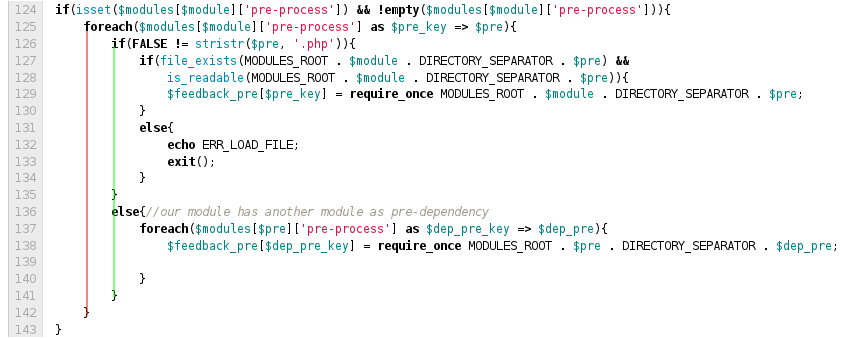
\includegraphics[scale=.5]{cap02/code_align.png}
  \caption{Alinierea codului}
  \label{fig:code_align}
\end{figure}

Observi cum liniile 125 și 142 sunt aliniate vertical. La fel și 126 și 141. Astfel ochiului uman (cu puțin de antrenament)
îi este foarte ușor să își dea seama care acoladă cui aparține.

În continuare, toate listările vor respecta în continuare aceeași convenție de formatare a codului
în mod consistent. Nu vor mai fi introduse explicit unele convenții, însă este bine să fii atent
la aceste detalii pe măsură ce avansezi.

Încă o mică convenție nescrisă: identificatorii \texttt{foo} și \texttt{bar} sunt folosiți ca înlocuitori
pentru ceva fără semnificație. În cazul lor, programatorul vrea să sublinieze că nu variabilele respective
în sinea lor sunt importante, ci alte concepte atașate lor.

\section{Input și formulare}
Atunci când utilizatorul introduce date, pe care le numim colectiv \textsl{input},
acele date trebuie salvate în ceva pentru a avea acces la acele date. Iar cel
mai la îndemână loc de a le salva sunt variabilele.

Una dintre variabilele în care PHP salvează automat un anumit tip de input este \get.
Pentru a o popula cu valori, un utilizator trebuie să introducă ceva în \textsl{request line}-ul
cererii HTTP.

Deci crează un script \texttt{get.php} cu următorul conținut, ca să vezi ce conține variabila \get:
\begin{lstlisting}
<?php
var_dump($_GET);
\end{lstlisting}
Apoi crează o cerere HTTP cu telnet:
\begin{verbatim}
GET /get.php HTTP/1.1
Host: localhost

\end{verbatim}
Întreaga comunicație va arăta cam așa:
\begin{verbatim}
GET /webdev/get.php HTTP/1.1
Host: localhost

HTTP/1.1 200 OK
Date: Sun, 06 Jun 2010 20:27:40 GMT
X-Powered-By: PHP/5.3.2
Content-Length: 13
Content-Type: text/html

array(0) {
}
\end{verbatim}
Observăm că {\get} este un array, și că are zero elemente. Altfel spus,
e un array gol. Ceea ce e logic, din moment ce nu pare să fi făcut niciun
pas special pentru a introduce date. Pentru a introduce date cu metoda GET,
trebuie să creăm parametri pe care să-i adăugăm la adresa resursei cerute.
Sintaxa generală este:
\begin{verbatim}
'/path/to/script.php' ['?' <name> '=' <value> ['&' <name> '=' <value>]+ ]
\end{verbatim}
În cuvinte: numele resursei este urmat de semnul întrebării, apoi o serie de
una sau mai multe perechi nume {\glqq}ia valoarea{\grqq} valoare, separate de caracterul
ampersand ('\&').

Deci fă cererea HTTP:
\begin{verbatim}
GET /get.php?foo=bar&answer=42
\end{verbatim}

Vei vedea că \get\ are valoarea:
\begin{verbatim}
array(2) {
  ["foo"]=>
  string(3) "bar"
  ["answer"]=>
  string(2) "42"
}
\end{verbatim}
După cum observi, nu e nimic special la \get, este un array asociativ
cu care putem lucra așa cum am lucrat cu toate array-urile de până acum.
Cheile din array sunt numele parametrilor, iar valorile \ldots Valorile sunt
mereu stringuri!

Asta nu este neapărat un lucru rău, PHP ne scapă de necesitatea de a converti
(cu type casting) explicit atunci când detectează că poate face o conversie
automată, însă mult mai bine este să convertim noi toate inputurile.

PHP decide cum trebuie să convertească anumite tipuri de date în alte tipuri
de date în funcție de \textit{contextul semantic} în care punem acele date. De exemplu
o valoare 'ABC' în contextul semantic al unei expresii booleene este evaluată
ca TRUE.

\attention{Pentru a valida cu adevărat inputul, va trebui să folosim funcții,
însă funcțiile vor fi prezentate abia în capitolul 3. Deci deocamdată ne
prefacem că un simplu type casting și câteva verificări sunt suficiente.
Facem asta pentru a ne educa din start cu ideea necesității validării inputului.

Tehnici de validare complete vor fi prezentate după introducerea funcțiilor.}

Deci vom putea face un calculator care adună două numere a și b
introduse de utilizator, și afișează rezultatul adunării:
\begin{lstlisting}
<?php
echo (int)$_GET['a'],' + ', (int)$_GET['b'], ' = ', $_GET['a'] + $_GET['b'];
\end{lstlisting}
Vizitează adresa \texttt{http://localhost/add.php?a=3\&b=4}.

Dar oare ce se întâmplă atunci când unul dintre parametri este inexistent?
Hai să vedem. Vizitează direct \texttt{http://localhost/add.php}. PHP îți
va spune ce ai greșit. Mesajul în browser este dificil de citit, deci
folosește opțiunea {\glqq}view source{\grqq} a browserului tău. În firefox, poți apăsa
\keystroke{CTRL+U}.

PHP ne spune ceva de genul
\begin{verbatim}
Undefined index: a in add.php on line 2
\end{verbatim}
pentru fiecare acces la indexul (cheia) 'a' respectiv 'b'
de pe linia 2. Astfel de mesaje ar putea fi utile unui
atacator care ar putea deduce din mesajele afișate cam cum
arată codul tău sursă. Ar putea folosi acele deducții pentru
a-ți sparge site-ul.

Din acest motiv vrem să verificăm mai întâi
dacă cheile 'a' respectiv 'b' există într-adevăr în \get\ \textit{înainte}
de a accesa acei membri ai array-ului. Dacă ambii membri 'a'
și 'b' nu sunt prezenți, atunci afișăm un mesaj de eroare,
altfel facem calculele, pentru că avem cu ce. În acest fel,
orice ar introduce un eventual atacator, acesta nu ar
vedea informații importante pentru el pe care noi nu vrem
să le dezvăluim despre codul nostru sursă:
\begin{lstlisting}[label=lst:addition,caption={Un calculator simplu}]
<?php
if(!isset($_GET['a']) || !isset($_GET['b'])) {
  echo 'Introdu a si b.';
}
else {
  echo (int)$_GET['a'],' + ', (int)$_GET['b'], ' = ', $_GET['a'] + $_GET['b'];
}
\end{lstlisting}
După cum știi, operatorul de negație în PHP este !. El inversează practic valoarea
de adevăr a expresiei logice care urmează. În cazul nostru inversează
valoarea de adevăr a constructului isset(),
care are în interior pe rând parametrii \verb|$_GET['a']| respectiv  \verb|$_GET['b']|.
\begin{Exercise}[title={Înțelege expresia logică},difficulty=1]
\ExePart
Cum se citește linia 2 din listingul \ref{lst:addition}? Începe răspunsul așa:\\
\textit{Dacă \ldots}.

\ExePart

Rescrie condiția într-o formă {\glqq}mai compactă{\grqq} folosind legile lui De Morgan.
Explică încă o dată cum se citește această nouă linie de cod, așa cum
ai făcut în partea I a exercițiului pentru condiția inițială.
\end{Exercise}

\good{Mereu caută să-ți rescrii expresiile logice cu ajutorul
legilor lui De Morgan astfel încât să conțină cât mai multe conjuncții logice.
Asta îți va face scriptul mai rapid, deoarece într-o conjuncție logică, de îndată
ce s-a întâlnit o valoare FALSE, expresiile următoare din acea conjuncție
nu mai sunt evaluate, pentru că nu mai are rost: întreaga conjuncție logică
va avea oricum valoarea de adevăr FALSE.

Deci dacă în exemplul nostru ar fi mai probabil să nu existe 'b', dar să existe 'a',
atunci ar fi mai bine să verificăm mai întâi dacă 'b' este setat. Asta ne-ar economisi
nevoia de a-l verifica și pe 'a'.

În exemplul nostru micuț nu este neapărat cazul, șansele statistice ca un
utilizator răuvoitor să nu seteze ori 'a' ori 'b' sunt practic egale. Însă reține
această modalitate de optimizare pentru situațiile mai complexe.

De exemplu, de preferat ar fi să verifici mai întâi unele variabile introduse de
utilizator, și abia apoi să verifici conjunctiv valori dintr-o bază de date, deoarece
operațiile precum căutările în baze de date sunt mult mai scumpe în termeni
de performață.
}

\begin{Exercise}[title={Un calculator complet},difficulty=2]
Crează un script care acceptă doi parametri obligatorii 'a' și 'b' și un parametru
opțional 'op' care ia ca valori 'add', 'sub', 'mul', 'div' sau 'mod' pentru fiecare
dintre operațiile adunare, scădere, înmulțire, împărțire și modulo.

Dacă parametrul 'op' nu este specificat, atunci trebuie să calculeze rezultatul
tuturor operațiilor $a+b,a-b,a*b,a/b$ și $a\%b$ și să le afișeze rezultatul. Dacă este
specificat, scriptul trebuie să calculeze doar operația corespunzătoare și
să-i afișeze rezultatul.

Folosește constructul \texttt{switch} pentru a decide ce operație trebuie să faci.
Provocarea constă în a nu scrie cod repetitiv.

\textit{Cod repetitiv} înseamnă că ai o secvență de una sau mai multe instrucțiuni identice
în mai multe locuri din algoritm.
\end{Exercise}

\subsection{Formulare, business logic și view logic}

Însă utilizatorul de rând nu ar trebui să aibă cunoștințe tehnice pentru a-ți
trimite date către procesare. Pentru asta există formulare HTML.

Numele câmpurilor de input (atributul \texttt{name}) vor fi folosite \textit{de browser}
pentru a genera URL-ul corect, dacă formularul este
trimis prin metoda GET. De exemplu, un script de întâmpinare a
vizitatorului ar putea arăta astfel:
\begin{lstlisting}
<?php
$mesaj = NULL;
if(isset($_GET['submit'])) {
  if(isset($_GET['nume']) && $_GET['nume']) {
	$mesaj = 'Salut '.$_GET['nume'];
  }
  else {
	$mesaj = 'Eroare: Nu ai introdus numele.';
  }
}
echo $mesaj;
?>
<form method="get">
<label for="nume">Nume:</label>
<input type="text" name="nume" id="nume" />
<input type="submit" name="submit" value="saluta-ma" />
</form>
\end{lstlisting}
Scriptul este constituit din două părți: liniile 2-10 se ocupă de procesarea
formularului. Liniile 11-17 se ocupă de generarea outputului pe baza datelor
procesate.

Transmiterea de informații din procesare către generarea de output se face
folosind \textsl{variabila intermediară} \$mesaj. Deoarece ea va avea ca valoare un
string, o inițializăm cu valoarea NULL, pe linia 2.

Dacă condiția de pe linia 3 este adevărată, înseamnă că utilizatorul a apăsat
butonul {\glqq}submit{\grqq}. În acest caz, vrem să procesăm formularul.

Indiferent
dacă formularul a fost trimis sau nu, 
afișăm direct mesajul, care e NULL dacă formularul nu a fost trimis, deci nu rezultă niciun output în
urma executării liniei 11, și afisăm și formularul.

Dacă formularul nu a fost trimis, atunci cel mai probabil vizitatorul tocmai a intrat
pe pagina noastră și urmează să-l completeze și să-l trimită.

Linia 4 verifică dacă \texttt{\$\_GET['nume']} este setat, și dacă da, verifică
și dacă valoarea salvată în el este evaluată boolean ca fiind TRUE. Altfel spus,
verifică și dacă stringul nu este gol (\texttt{''}) sau nu are valoarea '0'.

Dacă toate acestea sunt adevărate, se generează o valoare dinamică ca mesaj de salut pe linia 5.
Altfel valoarea dinamică va fi un mesaj de eroare, inițializat pe linia 8.

Procesarea formularului de pe liniile 2-10 se numește și \textsl{business logic}.
Acea secvență
din cod validează inputul și setează variabila intermediară \$mesaj în concordanță
cu acest input, sau cu absența inputului.

Variabila intermediară \$mesaj salvează în ea ceea ce numim {\glqq}informație atomară a aplicației{\grqq}.
Se numește așa deoarece, cel puțin în scriptul nostru, constituie o bucățică de informație
indivizibilă, de sine stătătoare.

Generarea outputului pe baza variabilelor intermediare (aici liniile 11-17) constituie
\textsl{view logic} -- logica de vizualizare.

Am fi putut genera output și direct pe liniile 5 respectiv 8, inclusiv formularul,
însă separând \textsl{business logic} de \textsl{view logic},
putem modifica și adapta mai ușor scriptul la noi nevoi.

Logica din spatele aplicației nu are nimic de-a face cu modul ei de prezentare, iar
asta ar trebui să fie reflectat și de codul însuși. Una este validarea inputului,
alta este afișarea.

Mai târziu vei vedea că vei putea genera tot felul de formate de output, nu numai HTML,
cu mai multă ușurință, deoarece business logic va rămâne același, și va trebui
doar să introduci un nou view logic pe baza variabilelor intermediare pe care business logic
ți le pune la dispoziție.

\good{Separă view logic de business logic și introdu variabile intermediare exact
acolo unde este nevoie, variabile care salvează doar informațiile atomare de la baza
aplicației.}

\begin{Exercise}[title={View Logic și Business Logic},difficulty=1]
Îmbunătățește scriptul scris ca soluție la exercițiul {\glqq}Un calculator complet{\grqq},
adăugând un formular care să fie trimis prin metoda POST în loc de GET.

Datele trimise prin POST sunt puse de PHP în array-ul \texttt{\$\_POST}.

Separă business logic de view logic, exact ca în exemplul anterior, folosind
variabile intermediare.
\end{Exercise}

\bad{Deși poți salva valori în array-uri precum \get sau \texttt{\$\_POST}, nu
este bine să o faci. Array-uri ca acestea sunt gândite pentru a prelua
input de la utilizator, sunt populate automat de PHP.

Altfel spus, ele au semantica de input, deci nu ar trebui să le încalci
semantica salvând datele tale proprii în ele.}

%FIXME explicatiile despre VL si BL din 12 ian. 2011 ora 18:25 de pe IRC

\section{Array-uri multidimensionale}
Array-urile sunt structuri de date compozite în care putem salva valori.
Însă un array însuși este o valoare. Din asta deducem inductiv că
putem avea array-uri în array-uri.

Un array bidimensional are două dimensiuni, și ar putea fi inițializat
astfel:
\begin{lstlisting}
$array_2d = array(
  array('foo'),
  array('bar')
);
echo '<pre>';
var_dump($array_2d);
echo '</pre>';
\end{lstlisting}
Bineînțeles că putem refolosi variabile în care am salvat anterior array-uri
pentru a crea noi array-uri. De exemplu, un array tridimensional ar putea arăta
astfel:
\begin{lstlisting}
$array_3d = array(
  'one' => $array_2d,
  'two' => $array_2d
);
var_dump($array_3d);
\end{lstlisting}
Putem crește oricât în dimensiuni, sau putem chiar avea un array cu dimensiuni variabile:
\begin{lstlisting}
<?php
$array_multidim = array(
  $array_2d,
  array('inner 2d' => $array_2d,$array_3d),
  $array_2d
);
var_dump($array_multidim);
\end{lstlisting}

După cum știi deja, array-urile sunt îndeosebi utile atunci când vrem să procesăm anumite date
cu același (sub)algoritm.

Un exemplu pragmatic ar fi să-i cerem utilizatorului să bifeze fructele sale preferate,
și pe baza lor să afișăm anumite informații despre ele.

În formularul HTML nu va trebui decât să numim câmpurile de input cu {\glqq}[]{\grqq}, exact așa cum
am accesa și array-urile în PHP. Pentru o serie de checkbox-uri am putea avea:
\begin{lstlisting}[language=HTML]
<form method="POST">
  <input type="checkbox" name="fructe[]" value="mere" />
  <input type="checkbox" name="fructe[]" value="pere" />
</form>
\end{lstlisting}
Am putea și denumi acele intrări dacă în PHP semantica datelor nu este
de o înșiruire, ci un set de date asociative:
\begin{lstlisting}[language=HTML]
<form method="POST">
  <input name="fructe[mere]" />
  <input name="fructe[pere]" />
</form>
\end{lstlisting}

Un exemplu complet pentru un astfel de script ar putea arăta astfel:
\begin{lstlisting}[label=lst:favourite-fruits,caption={Fructe favorite}]
<?php
$fructe = array(
  'mere' => 'Merele contin multi antioxidanti.',
  'pere' => 'Perele sunt bogate in vitamina C si in potasiu.',
  'alune' => 'Alunele sunt bogate in proteine, grasimi nesaturate si vitamina B6.'
);
if(isset($_GET['submit']) && isset($_GET['fructe'])) {
  foreach($_GET['fructe'] as $fruct) {
	echo '<p>',$fructe[$fruct],'</p>';
  }
}
?>
<form method="GET">
  <input type="checkbox" name="fructe[]" value="mere" id="mere-id" /> <label for="mere-id">Mere</label>
  <input type="checkbox" name="fructe[]" value="pere" id="pere-id" /> <label for="pere-id">Pere</label>
  <input type="checkbox" name="fructe[]" value="alune" id="alune-id" /> <label for="alune-id">Alune</label>
  <input type="submit" name="submit" value="Trimite" />
</form>
\end{lstlisting}

Liniile 14-16 sunt foarte repetitive, și deși putem proceda ca în exemplul de mai sus punând câte un
checkbox, un label, și o intrare în array-ul \$fructe care conține informațiile efective, acest lucru e foarte
ineficient și mănâncă timp dacă vrem să personalizăm acest script.

\good{Când ai linii de cod repetitive foarte asemănătoare din punct de verede structural,
cel mai probabil poți face acele lucruri într-o buclă. Folosește aceste bucle pentru a
reduce costurile de mentenanță (și modificare) a codului, deci implicit și pentru
economisirea timpului. Astfel devii mai productiv.}

Ce se întâmplă dacă vrem să adăugăm sau
să ștergem un fruct? Trebuie să o facem în trei locuri!

Practic însă avem toate informațiile de care avem nevoie (lista de fructe posibile) în array-ul \$fructe,
deci putem folosi acele informații pentru a genera formularul HTML.

\begin{Exercise}[title={Structuri de date abstracte},difficulty=1]
Modifică scriptul din listingul \ref{lst:favourite-fruits} astfel încât să genereze dinamic
formularul HTML pe baza structurii de date asociative \$fructe.

Îmbunătățește scriptul astfel încât să nu dea erori pentru inputuri precum\\
\texttt{/fructe.php?fructe[]=capsuni\&submit=Trimite}
\end{Exercise}

\good{După cum observi, deja ai învățat o grămadă de lucruri care îți pot
ușura munca și economisi timp și îți oferă și flexibilitate.

Tot ce trebuie acum să faci e să reflectezi asupra lucrurilor învățate și să îți
imaginezi cum le-ai putea combina.

Ai la dispoziție variabile și structuri de date, ramificări condiționale ale
fluxului de execuție, și bucle.
}

\subsection{Geometria și normalizarea array-urilor}
Geometria unui array descrie felul în care arată un array. O caracteristică
a geometriei este numărul de dimensiuni a array-ului și/sau a fiecărui câmp.

De exemplu putem stabili că un câmp \texttt{pasiuni} este o listă de pasiuni,
deci pe undeva în aplicație putem avea:
\begin{lstlisting}
$pasiuni = array('tenis', 'fotbal', 'balet');
\end{lstlisting}

Structurile\footnote{Array-urile} de date pot crește însă în complexitate, de
exemplu putem descrie o persoană cu următoarea listă de meta-date:
\begin{lstlisting}
$persoana = array(
  'nume' => 'Xulescu',
  'varsta' => 15,
  'liceu' => 'George Enescu',
  'pasiuni' => array('tenis', 'fotbal', 'balet')
);
\end{lstlisting}
Meta-datele precum \texttt{nume} sau \texttt{pasiuni} sunt fixe, dar valorile
pot varia de la om la om. Cert este că un câmp \texttt{varsta} va fi mereu
integer, iar \texttt{pasiuni} va fi mereu un array.

Dar ce se întâmplă dacă o persoană nu are pasiuni? Simplu: lista de pasiuni
poate fi goală:
\begin{lstlisting}
$persoana = array(
  'nume' => 'Xulescu',
  'varsta' => 15,
  'liceu' => 'George Enescu',
  'pasiuni' => array()
);
\end{lstlisting}
În acest fel, chiar dacă nu avem pasiuni, structura de date în întregimea sa
respectă în continuare geometria prestabilită a array-ului.

Ce se întâmplă dacă în cadrul aplicației noastre stabilim și că
o persoană poate avea și caracteristici precum \texttt{facultate}
sau \texttt{limbi\_cunoscute}? Va trebui să adăugăm și aceste caracteristici,
pentru a păstra array-ul normalizat, chiar dacă persoana respectivă nu are
o anumită \texttt{facultate} drept caracteristică.

Obținem:
\begin{lstlisting}
$persoana = array(
  'nume' => 'Xulescu',
  'varsta' => 15,
  'liceu' => 'George Enescu',
  'facultate' => NULL,
  'limbi_cunoscute' => array('romana'),
  'pasiuni' => array()
);
\end{lstlisting}

Atunci când aducem o structură de date la cea mai complexă formă a sa,
spunem că am \textsl{normalizat} acea structură, sau că am adus-o la o \textsl{formă
canonică}.

\section{Sisteme de numerație}
\subsection{Baze numerice}
Pentru a înțelege operațiile binare, trebuie să înțelegem mai întâi sistemele
de numerație.

Primul sistem de numerație pe care l-ai învățat și cu care te simți cel
mai confortabil este sistemul decimal. Se numește astfel deoarece
ai la dispoziție zece simboluri, fiecare din ele reprezentând o cantitate:
0, 1, 2, 3, 4, 5, 6, 7, 8, 9.

Trebuie să facem însă distincția clară între cantitate și reprezentarea
acesteia. În cazul nostru, cantitatea doisprezece are reprezentarea 12.

Dar ce se întâmplă când numărăm? Cum numărăm de fapt? Ai învățat
asta când erai copil și ți-a intrat atât de adânc în procesele cognitive,
încât nici nu mai poți conștientiza ce faci când numeri de fapt.

Când numeri, iei pe rând simbolurile pe care le ai la dispoziție 0, 1, 2, 3, 4, 5, 6, 7, 8.
O dată ajuns la 9, nu mai ai simboluri, deci adaugi unu la poziția imediat din
stânga, și încă unul la poziția la care ești, în cazul nostru la poziția unităților.

Asta e posibil deoarece reprezentarea
\begin{verbatim}
9
\end{verbatim}
este același lucru cu
\begin{verbatim}
09
\end{verbatim}
sau cu oricâți de 0 în față, nu contează:
\begin{verbatim}
00000009
\end{verbatim}
Deoarece după ultimul simbol, în cazul nostru 9, urmează primul simbol, deci 0, și invers,
deoarece înaintea lui 0 se află simbolul 9, spunem că acest șir de simboluri
0, 1, 2, 3, 4, 5, 6, 7, 8, 9, este un \textsl{șir circular}. Ca o analogie
la ce înseamnă \textit{circular}, gândește-te la un lacăt cu cifru.
Așa se face că după 009 urmează 010, adică zece.

Până acum am numărat în baza 10. Acum hai să generalizăm. Să zicem că avem
simbolurile s,t,u,v, și vrem să numărăm crescător în baza 4, deoarece avem
patru simboluri. Pentru asta nu trebuie decât să luăm simbolurile la rând:
\texttt{s}, \texttt{t}, \texttt{u}, \texttt{v}.
O dată ajunși la \texttt{v}, nu mai avem simboluri, deci trebuie să sărim
pe poziția următoare și să adăugăm cantitatea 1.

Cum pe poziția următoare
se află s (similar cu acel 0 {\glqq}invizibil{\grqq} din baza 10), și deoarece după v
urmează s, deducem că după \texttt{v} urmează \texttt{ts}, care reprezintă
deci cantitatea 4. În continuare ar urma
\texttt{tt}, \texttt{tu}, \texttt{tv}, 
\texttt{us}, \texttt{ut}, \texttt{uu}, \texttt{uv}, \ldots, vv, \ldots,
\texttt{tss}, \texttt{tst}, \texttt{tsu}, \texttt{tsv},
\texttt{tts}, \texttt{ttt}, \ldots, \texttt{vvs}, \texttt{vvt},
\texttt{vvz}, \texttt{vvv}, \texttt{tsss}, \ldots

\begin{Exercise}[title={Numără în baza șapte},difficulty=2]
Numără până la cantitatea două zeci în baza șapte folosind setul
de simboluri ordonate d, g, h, a, s, z, u.
\end{Exercise}

Orice bază de numerație, fie ea binară (2), octală (8) sau
hexadecimală (16) funcționează după exact aceleași principii.

Demn de menționat este că în PHP, valorile pot fi introduse
folosind reprezentarea lor octală punând zero în fața lor, iar
valorile hexadecimale pot fi introduse direct prefixându-le cu 0x.
Pentru reprezentarea hexadecimală se folosesc pe rând literele A, B, C,
D, E, F care urmează după simbolul 9.
Exemple:
\begin{lstlisting}
<?php
$foo = 052;
echo $foo,' ', 0x2A;
\end{lstlisting}

\subsection{Operații pe biți}
Există șase operații binare în PHP, iar înțelegerea lor este
foarte ușoară dacă ai înțeles deja expresiile booleene și
operațiile logice prezentate în paginile
\pageref{sec:tipul de date boolean. Expresii logice}--\pageref{endsec:tipul de date boolean. Expresii logice}.

Plecând de la reprezentarea binară a două cantități, de exemplu \texttt{00101010} și
\texttt{01100111}, putem uni conjunctiv fiecare bit cu bitul corespunzător din a doua valoare.
1 este același lucru cu TRUE iar 0 același lucru cu FALSE din tabelul \ref{tbl:truth table and or}.
Această operație se numește \textsl{binary and}, iar operatorul PHP este \texttt{\&}.
Calculăm:
\begin{verbatim}
00101010 &
01100111
--------
00100010
\end{verbatim}

Operația disjunctivă se numește \textsl{binary or}, și are operatorul |. Calculăm:
\begin{verbatim}
00101010 |
01100111
--------
01101111
\end{verbatim}

Mai putem muta și la dreapta șirul de biți cu un număr de poziții. Operatorul
pentru asta este \texttt{$>>$} și se numește \textsl{shift to right}. Exemplu:
\begin{verbatim}
00101010 >> 3 = 00000101
\end{verbatim}

Un octet (en. \textsl{byte}) este un șir de opt biți,
iar un bit este 0 sau 1. În exemplele de mai sus am făcut deci operațiile binare
\textit{and} și \textit{or} pe reprezentarea într-un byte a doi operanzi.

În PHP, numerele întregi ocupă un anumit număr de bytes. Acesta este dependent de
platformă, și este de obicei 4 sau 8. Află cât spațiu au la dispoziție numerele
întregi:
\begin{lstlisting}
<?php
echo PHP_INT_SIZE,PHP_EOL;
\end{lstlisting}

Acum știm tot ce trebuie pentru a afișa reprezentarea binară a oricărui număr:
\begin{lstlisting}[label=lst:bitbybit,caption={Afișarea bit cu bit a unui int}]
<?php
$a = 42;
for($i=8*PHP_INT_SIZE-1;$i>=0;$i--) {
  echo ($a>>$i) & 1 ? '1':'0';
}
\end{lstlisting}

\attention{În urma operației \textit{shift to right} cu X biți, se pierd cei mai din
dreapta X biți, iar în partea din stânga X biți (care apar {\glqq}noi{\grqq}) sunt inițializați
cu zero.}

\begin{Exercise}[difficulty=3,title={Cum funcționează afișarea bit cu bit a unui int?}]
Explică cum funcționează codul din listingul \ref{lst:bitbybit}.

Concentrează-te
în special pe expresia \texttt{(\$a$>>$\$i) \& 1}.

Experimentează și fă observații pe baza experimentelor. Ai putea citi și articolul
de pe wikipedia.\footnote{\url{http://en.wikipedia.org/wiki/Bitwise_operation}}
\end{Exercise}

Analog cu \textit{shift to right}, există și un \textsl{shift to left}. Operatorul este
\texttt{$<<$}, după cum poți vedea \^in listingul \ref{lst:shiftleft}.
\begin{lstlisting}[label=lst:shiftleft,caption={Operatorul shift to left}]
<?php
$a = 42;
for($i=8*PHP_INT_SIZE-1;$i>=0;$i--) {
  echo ($a>>$i) & 1 ? '1':'0';
}
$a <<= 5;
echo PHP_EOL;
for($i=8*PHP_INT_SIZE-1;$i>=0;$i--) {
  echo ($a>>$i) & 1 ? '1':'0';
}
\end{lstlisting}
După cum observi pe linia 6, putem contracta operațiile binare cu operația de atribuire
într-o singură operație.

Similar cu shift to right, biții din dreapta sunt inițializați automat cu 0, iar cei din
stânga se pierd. 

O altă operație este \textsl{inversarea} sau \textsl{negarea} biților. 0 devine 1, iar 1 devine 0.
În contrast cu operațiile de până acum, inversarea biților\footnote{La fel ca negarea
booleană, unde !<expr> are valoarea de adevăr inversă a expresiei.} are un singur operand.
Operatorul este $\sim$ și se pune în fața operandului: 
\begin{lstlisting}
<?php
$a = 42;
for($i=8*PHP_INT_SIZE-1;$i>=0;$i--) {
  echo ($a>>$i) & 1 ? '1':'0';
}

echo PHP_EOL;
$a = ~42;
for($i=8*PHP_INT_SIZE-1;$i>=0;$i--) {
  echo ($a>>$i) & 1 ? '1':'0';
}
\end{lstlisting}

Ultima operație binară este \textsl{exclusive or}, sau pe scurt
\textsl{xor}. Operatorul este \textasciicircum, și
acceptă doi operanzi. În algebră booleană, am descrie această operație așa:
\[(\lnot a \land b) \lor (a \land \lnot b)\]

\begin{Exercise}[title={Jonglează cu expresii boolene},difficulty=3]
Explică în limba română, pe baza definiției operației xor
$(\lnot a \land b) \lor (a \land \lnot b)$,
în ce situații este foarte utilă această operație.
\end{Exercise}


%TODO modifica acest exercitiu, adauga mai multe explicatii,
% probabil va trebui sa transform exercitiul in explicatii din text,
% iar exercitiul sa devina "rescrie a.i. sa fie shift-uit 1, nu inputul" (catch: nu se va spune
% ca trebuie shiftuit la stanga)
\begin{Exercise}[title={Operații pe biți}]
Crează un script care acceptă două numere a și b, cu b mai mic sau egal cu 8*PHP\_INT\_SIZE-1, și
care afișează rezultatele operațiilor \texttt{a\&b}, \texttt{a|b}, \texttt{a$<<$b},
\texttt{a$>>$b}, \texttt{a{\textasciicircum}b},
\texttt{{\texttildelow}a}, \texttt{{\texttildelow}b} și \texttt{(a$>>$b)\&0x1}.
\end{Exercise}

Operațiile pe biți sunt foarte utile atunci când vrem să setăm atribute booleene {\glqq}da sau nu{\grqq}
pentru anumite proprietăți, drepturi de acces, etc. Avantajul este că aceste câmpuri de biți
(en. \textsl{bitfields}) sunt foarte compacte, ocupă puțin spațiu.

Un scenariu de utilizare:
\begin{lstlisting}
<?php
const AUTH_NONE = 0x00;
const AUTH_READ = 0x01;
const AUTH_WRITE = 0x02;
const AUTH_DELETE = 0x04;

$drepturile_mele = AUTH_READ|AUTH_WRITE|AUTH_DELETE;

if($drepturile_mele & (AUTH_READ|AUTH_WRITE)) {
  echo 'poti citi si scrie<br>';
}
\end{lstlisting}
Liniile 2-5 inițializează constante cu drepturile respective.  Cantitățile 1, 2 și 4
au fiecare biții doar câte un bit setat, de la dreapta la stânga, 1 are primul bit setat,
2 are al doilea bit setat, 4 îl are doar pe al treilea setat. Astfel nu avem conflicte
între cele patru niveluri de acces. Folosim constante
deoarece acei biți nu se schimbă niciodată.

Linia 7 unește conjunctiv toate drepturile de acces, ceea ce rezultă practic în șirul
de biți \texttt{00000111}.

Linia 9 verifică conjunctiv dacă drepturile utilizatorului care vizitează
momentan pagina include și bitul AUTH\_READ. După evaluarea condiției
de pe linia 9 ne alegem fie cu valoarea 0, fie cu o altă valoare,
care conform observațiilor pe care le-ai făcut în listingul \ref{lst:typecasting}
va fi evaluată ca TRUE.

Teoretic am fi putut folosi și un array asociativ, de exemplu:
\begin{lstlisting}
<?php
$drepturile_mele = array(
  'read' => TRUE,
  'write' => TRUE,
  'delete' => TRUE
);
if($drepturile_mele['read'] && $drepturile_mele['write']) {
  echo 'poti citi si scrie<br>';
}
\end{lstlisting}
însă ocupă mult mai mult spațiu și nu este la fel de compact.
În plus, bitfield-urile pot fi salvate mult mai ușor în alte
sisteme precum baze de date, poți sorta după anumite valori, ș.a.m.d.

\section{Variabile variabile}
O variabilă variabilă se numește astfel deoarece îi construim numele (identificatorul) variabil,
pe baza altor valori. Pentru a crea o variabilă variabilă, folosim \$, urmat de identificatorul unei variabile,
care după cum știm, începe tot cu \$. Deci ne alegem cum două simboluri \$\$ unul după altul.

Exemplu:
\begin{lstlisting}
<?php
$a = 'b';
$$a = 'c';
var_dump($b);
\end{lstlisting}
După cum observi, nu declarăm nicăieri o variabilă \$b, însă o folosim pe linia 4.
Variabila \$b este creată pe linia 3, pe baza valorii variabilei \$a.

Putem chiar crea variabile din array-uri asociative, de exemplu:
\begin{lstlisting}[label=lst:varvarfromassoc,caption=Variabile variabile din array asociativ]
<?php
$variabile = array(
  'foo' => 'bar',
  'foobar' => 'barfoo'
);
foreach($variabile as $nume => $valoare) {
  $$nume = $valoare;
}
echo "$foo $foobar";
\end{lstlisting}

Atunci când creăm o variabilă (variabilă sau nu, nu contează), PHP îi pune identificatorul și valoarea
într-un tabel. Acest tabel se numește \textsl{scopul global} de variabile (en. \textsl{variable global scope}).

Folosind variabile variabile, poluăm acest \textit{scope}, iar asta este o practică rea.
Există unele situații în care variabilele variabile sunt utile, dar acestea implică
alte \textit{scope}-uri, nu cel global. Un astfel de exemplu\footnote{Și singurul în care
folosirea variabilelor variabile este legitimă, după părerea autorului.} îl vom întâlni
în capitolul următor.

\section{Referințe}
După cum știi, variabilele create sunt salvate de PHP într-un tabel cu identificatorul
și valoarea variabilei.

Referințele sunt ca niște nume alternative pentru aceeași valoare. Pentru a crea o referință,
punem '\&' în fața identificatorului variabilei pe care vrem să o referențiem. Exemplu:

\begin{lstlisting}
<?php
$a = 42;
$b = &$a;
echo $a,' ';
$b++;
echo $a;
\end{lstlisting}
Conform liniei 3, identificatorul \$b va {\glqq}arăta cu degetul{\grqq} (en. \textsl{point at})
către conținutul variabilei \$a. Pe linia 5 incrementăm acea valoare, însă prin prisma
identificatorului \$b.

Din moment ce și \$a, și \$b, arată către aceeași intrare din tabelul
\textit{\textit{scope}-ului global}, lucrul care
se reflectă și asupra valorii variabilei \$a pe linia 6.

\section{Exerciții}

\begin{Exercise}[title={Terminologie},difficulty=1]
În acest capitol ai învățat o grămadă de termeni noi.
Folosind cuprinsul de la pagina \pageref{cuprins},
ia fiecare secțiune a acestui capitol la rând, și la fiecare
scrie \textit{cel puțin} un cuvânt sau expresie,
fie el în română sau în engleză. La termenii în română,
scrie și corespondenții englezești.

Gândește-te cât știai înainte de a citi acest
capitol. Cum te simți? Eu m-aș simți mândru.
Felicitări!
\end{Exercise}

\begin{Exercise}[title={Rezumat},difficulty=2]
Explică în cel puțin 500 de cuvinte cum funcționează lucrurile pe care le-ai învățat și înțeles în acest
capitol. Folosește propriile formulări (fără copy/paste), și folosește cât mai mulți termeni
pe care i-ai găsit în exercițiul anterior.

Încearcă să sintetizezi cât mai multe lucruri care nu au fost spuse explicit, dar pe care
le poți deduce. Fă brainstorming\footnote{\url{http://en.wikipedia.org/wiki/Brainstorming}}
cu tine însuți, analizează conceptele
pe care le explici în rezumat.

Încearcă să te gândești cât mai serios și să reflectezi
asupra celor învățate.
De exemplu, gândește-te și explică ce legătură are conceptul de \textit{context semantic} cu
restul noțiunilor învățate în acest capitol (spre exemplu noțiunea de \textit{expresie} în PHP,
fie ea booleană, matematică, sau cu stringuri).

Nu te teme să faci afirmații îndrăznețe pentru a arăta că știi să gândești \textit{out
of the box}, deci că ai potențialul de a fi inovativ. Chiar dacă afirmațiile vor
fi greșite, este foarte probabil să înveți lucruri noi, pentru că-i faci 
pe tutorii {\phpro} să te corecteze și automat să vină cu explicații din care
să înveți lucruri noi, sau care îți clarifică unele lucruri. Sau cine știe,
poate ai o întrebare a cărei răspuns e atât de complex încât îi blochezi
pe tutori :-)
\end{Exercise}

\begin{Exercise}[title={Language Reference}]
Acest capitol a încercat să îți ofere o imagine cât mai clară a conceptelor
de bază, însă e foarte probabil ca unele noțiuni ori să nu fi fost
abordate cu destul de multă atenție la detalii, ori să nu fi fost abordate deloc.

PHP este documentat foarte bine în ceea ce numim \textit{manualul PHP}. Adresa
sa oficială este \url{http://php.net/manual}.

Intră pe manualul PHP și urmează cu atenție toate paginile din capitolul
\textit{Language Reference}.\footnote{\url{http://php.net/langref}}

\good{Citește exclusiv versiunea engleză a manualului. Este cea mai actuală
și cea mai corectă versiune. NU citi traducerea sa în română. Astfel
te vei și obișnui să lucrezi cu engleza, ca un viitor profesionist.}

Găsește cel puțin 5 lucruri care nu au fost spuse în carte și pe
care le-ai putut înțelege în urma citirii acelui capitol din manual.
% backtick - execution operator
% @$array[$index] suprima erori dacă $index nu există
% <> este același lucru ca !=
% << si >> inseamna inmultirea cu 2
% variabile predefinite _SERVER, etc
\end{Exercise}

\begin{Exercise}[title={Scrie scripturi}]

\ExePart

Scrie trei scripturi, fiecare de cel puțin 50 de
LOCs,\footnote{Liniile goale sau care consistă doar din comentarii nu se calculează}
care să aibă în total peste 250 de LOCs, și să rezolve probleme practice sau care
te-au preocupat mereu sau probleme pe care ți le-ai pus pe parcursul studiului acestor
capitole.

Scripturile trebuie să genereze cod XHTML 1.1 curat, și să fie
validate cu succes de \href{http://validator.w3.org/}{validatorul W3C}.\footnote{http://validator.w3.org/}

Fi atent și la accesibilitatea formularelor și generează cod XHTML semantic. Nu uita
să separi \textit{business logic} de
\textit{view logic} și să folosești variabile intermediare.

Posibile probleme de rezolvat:
\begin{itemize}
  \item generează un tabel HTML pe baza unui array bidimensional asociativ și afișează
rândurile din tabel colorate alternativ cu două culori de fundal, pentru o mai bună accesibilitate
  \item citește o sumă de bani (RON) și afișează numărul minim de bancnote din
fiecare sumă: 1, 5, 10, 50, 100, 200, 500, cu care poți acoperi suma introdusă
\end{itemize}

Cere ajutorul comunității de pe {\phpro} acolo unde te blochezi.

\ExePart

Explică pas cu pas unui neprogramator ce face fiecare cod și cum o face.
Nu ai voie să folosești termeni tehnici, ci doar formulări pragmatice.

\end{Exercise}
